%\section{Results}
Thus far I have outlined all reconstruction-level inputs to our analysis including event selection, backgrounds and their estimation methods, and systematic uncertainties. Each of these components is critical to our final result and this section will focus on the methods used to use these to extract VBF $H\rightarrow WW^*$ cross-section measurements. 
\section{Statistical analysis}
\subsection{Likelihood functions}
This analysis rests on the estimation of a parameter $\mu$ which describes the statistical significance of our signal yield relative to its Standard Model prediction and in this particular analysis defines the signal cross-section and signal and background yields. We build a likelihood function $\mathcal{L}(\mu,\Theta)$ where the signal strength $\mu$ is a parameter of interest (POI) and nuisance parameters (NPs) $\Theta=\Theta_a,\Theta_b,...$ represent all relevant uncertainties. None of these values are known a priori so the likelihood is built to represent the probability of particular values for the POIs and NPs. The analysis uses a maximum likelihood estimator to find the inputs which maximize the likelihood or equivalently and more mathematically tractable, minimize the negative log of the likelihood. Here I will briefly outline how a likelihood function can incorporate regions of interest. This discussion uses \cite{cranmer2015practical} as a guide. First, the Poisson distribution $\mathcal{P}(n|\lambda)$ describes the probability of $n$ events with a true unknown yield $\lambda$:
\begin{equation}
\mathcal{P}(n|\lambda)= \lambda^n\frac{e^{-\lambda}}{n!}
\end{equation}
Next we can define a variable observable $x$ with probability density $f(x)$ hence with $n$ events the probability density of each is multiplied. The likelihood of $\lambda$ can now be written
\begin{equation}
\mathcal{L}(\lambda)=\mathcal{P}(n|\lambda)\prod_{\text{event}}^n f(x)
\end{equation}
Our likelihood also must take into account multiple regions (the signal region as well as the control regions) and so these likelihoods are multiplied together with their own distinct Poisson distributions
\begin{equation}
\mathcal{L}(\lambda)=\prod_r^{\text{regions}}(\mathcal{P}(n_r|\lambda_r)\prod_{\text{event}}^n f(x))
\end{equation}
A simultaneous fit maximizes this likelihood function and so produces yield $\lambda$ for each free parameter simultaneously. The $\lambda$ values here represent predicted yields where $\lambda_{r,b} = \mu \lambda_{\text{sig}}+\lambda_{\text{bkg}}$. Maximizing the overall likelihood is made simpler by applying the natural logarithm (as the products between Poisson distributions become summations) and negating the likelihood, so as to take advantage of minimizing software.  

Particle physics defines discovery with rigorous standards using hypothesis testing. The null hypothesis is considered $\mu=0$ and is considered ``background-only" while the alternative hypothesis is that there is a signal above this background. The probability that the null hypothesis is rejected (or that the signal is discovered) is defined using a $p$-value. The $p$-value can be converted to a number of Gaussian standard deviations and in high energy physics three $\sigma$ significance (or a $p$-value of $1.35 \times 10^{-3}$) shows evidence while a five $\sigma$ result ($p$-value $2.87\times10^{-7}$) is considered a discovery.

In this analysis we use HistFitter software which is compiled with RooStats, RooFit, and HistFactory to complete our likelihood fit. We calculate the signal VBF Higgs cross-section in the fiducial space defined with signal region cuts (described in Chapter 4) with a simultaneous fit of the signal and control regions. Each region has a different distribution used in the fit to maximize that samples' discrimination against all other events. Overall we include seven floating parameters: signal strength for $\mu_{VBF}$, $\mu_{TopWW}$, $\mu_{Z+jets}$, and $\mu_{ggF}$, $\mu_{ggF1}$, $\mu_{ggF2}$, and $\mu_{ggF3}$. Other backgrounds (fakes, $V/\gamma$, $VH$, and $ttH$) are included as fixed parameters in the fit. 

The background treatment differs depending on the particular region and sample. For $Z+$jets, a designated control region is used and so the yield in the signal region can be found by including a transfer factor which maps the yield in the $Z+$jets control region to its yield in the signal region. The ggF signal strengths are split and derived as in shown in Chapter 5. Transfer factors to extrapolate yields from one region to another are derived by normalizing to the MC simulation. For backgrounds estimated within the signal region (Top/$WW$) the transfer factor is used only to extrapolate using simulations in the control regions where the contributions enters (other than the signal region) and so uncertainties associated with transfer factors are reduced. For the backgrounds included as fixed parameters in the fit, their predicted MC value is used (in the case of $V\gamma$, $VH$, and $ttH$) and for fakes their data-driven estimate is used. 

Events in the $e\mu$ and $\mu e$ channels are combined in the analysis and the likelihood is defined as the product of the Poissonians over BDT output bins in the signal region multiplied by the product of Poissonians over discriminant distributions in the controls regions (ggF CRs, $Z+$jets CR and Top/WW CR- within the signal region). The likelihood can then be calculated: 

\begin{equation}
  \begin{aligned}
\mathcal{L}(\mu) = \displaystyle\prod_{j=0}^{N_{\text{sig BDT bins}}} \mathcal{P} (n_{j}|\lambda_r) \times \displaystyle\prod_{k=1}^{N_{\text{CR-bins}}} P(n_{k}|\lambda_b) \\
\qquad = \displaystyle\prod_{j=0}^{N_{\text{sig BDT bins}}} \mathcal{P} (n_{j}|\mu_s \lambda_{sig,j} + \displaystyle\sum_{n}^{N_{\text{bkg}}}\mu_b^{n} \lambda_{bkg}^{nj}) \times \displaystyle\prod_{k=1}^{N_{\text{CR-bins}}} P(n_{k}|\mu_s \lambda_{sig,k} + \displaystyle\sum_{n}^{N_{\text{bkg}}}\mu_b^{n} \lambda_{bkg}^{nk})
  \end{aligned}
\end{equation}

Here the signal and background strengths are denoted $\mu$ and yields $\lambda$. Sums over all backgrounds $n$ include $Z+$jets, top/$WW$, and ggF; the minor backgrounds and data-driven $W+$jets estimate are added to Poisson expectations as fixed parameters. The last important addition to this likelihood is that of the numerous nuisance parameters affecting the analysis. These parameters $\Theta$ come in two general types: systematics which do not affect the shape of discriminating variables and those that do. Flat systematics are constrained with a unit Gaussian and their effects are measured for $\Theta=\pm1$. Shape systematics are split into purely flat and shape components and are again constrained with a unit Gaussian though their effects are measured through $\nu_{\text{shape}}(\Theta)= 1+\epsilon\Theta$ where $\epsilon$ is determined by measuring $\nu_{\text{shape}}$ at $\Theta=\pm 1$. Adding nuisance parameters $\Theta$ our final likelihood can be written 
\begin{equation}
  \begin{aligned}
\mathcal{L}(\mu,\vec{\Theta}) = \displaystyle\prod_{j=0}^{N_{\text{sig BDT bins}}} \mathcal{P} (n_{j}|\mu_s \lambda_{sig,j} + \displaystyle\sum_{n}^{N_{\text{bkg}}}\mu_b^{n} \lambda_{bkg}^{nj}) \times \displaystyle\prod_{k=1}^{N_{\text{CR-bins}}} P(n_{k}|\mu_s \lambda_{sig,k} + \displaystyle\sum_{n}^{N_{\text{bkg}}}\mu_b^{n} \lambda_{bkg}^{nk})  \times
  \displaystyle\prod_{i=1}^{N_{\Theta_i}}G(\tilde{\Theta_i}|\Theta_i,1)
  \end{aligned}
\end{equation}
where $G(\tilde{\Theta_i}|\Theta_i,1) = \frac{1}{\sqrt{2\pi}}e^{\frac{(\tilde{\Theta}-\Theta)^2}{2}}$ is the unit Gaussian and $\tilde{\Theta}$ is an auxiliary measurement of $\Theta$.

The fit is performed for a signal region, three ggF control regions, a $Z+$jets control region, and a shared top/$WW$ control defined within the signal region estimated in one half of the binned region defined by the signal region discriminant. Table \ref{tab:regiondefinitions} summarizes the regions used with in the fit and their cuts. These are discussed in more detail in Chapters 4 and 5. 

\begin{table}[h!]
\begin{center}
\resizebox{\textwidth}{!}{
\begin{tabular}{|c|c|c|c|c|c|c|}
\hline
Signal region   & Top/$WW$ control region & $Z+$jets control region & ggF SR & ggF CR 1 & ggF CR 2 & ggF CR 3 \\
\hline
\multicolumn{6}{|c|}{$n_{jets} \geq 2$}   & $n_{jets} <2$ \\
\hline
\multicolumn{7}{|c|}{b-veto} \\
\hline
\multicolumn{4}{|c|}{CJV $\geq20$GeV} & CJV$\geq 20$GeV and OLV$=1$ or CJV$<20$GeV and OLV$\neq1$ & CJV$\geq 20$GeV & - \\
\hline
\multicolumn{4}{|c|}{OLV$=1$} & - & OLV$\neq1$ & - \\
\hline
\multicolumn{2}{|c|}{$m_{\tau\tau}<m_Z-25$ GeV} & $|m_{\tau\tau}|-m_Z\leq 25$GeV &\multicolumn{4}{|c|}{$m_{\tau\tau}<m_Z-25$GeV} \\
\hline
\multicolumn{2}{|c|}{$m_{jj}>00$ GeV} & $m_{\ell\ell}<80$GeV & \multicolumn{4}{|c|}{$m_{jj}>00$ GeV} \\
\hline
\multicolumn{2}{|c|}{$\Delta Y_{jj}>2.1$}     & - & \multicolumn{4}{|c|}{$\Delta Y_{jj}>2.1$} \\
\hline
BDT$_{\text{VBF}} \geq 0$  & BDT$_{\text{VBF}} < 0$ & -0.5$<$BDT$_{\text{VBF}}>0.0$ & -  & -  & - \\
\hline
\end{tabular}}
\end{center}
\caption{Summary of all signal and control regions included in simultaneous fit}
\label{tab:regiondefinitions}
\end{table}

Each of the regions included in the fit uses a different discriminant to best characterize that sample's contribution. These discriminants are almost all BDT outputs trained on various kinematic distributions to characterize certain background and signal samples. These are discussed in Chapters 4 and 5. The $Z+$jets control region is defined with $m_T$ instead of a designated BDT after studies showed its success at mitigating uncertainty on $\mu_{Z+\text{jets}}$. These studies are included in Appendix A. Table \ref{tab:fitinputs} summarizes the regions used in the fit and shows their discriminant and number of bins. Table \ref{tab:cryields} shows MC event yields in all regions included in the fit. 
\begin{table}[!h]
  \begin{center}
    \begin{tabular}{l|cccccc}
       Category		& SR 	& Top/$WW$ CR 	& $Z+$jets CR 	& ggF-SR & ggF-CR1 		& ggF-CR2 	& ggF-CR3 \\
      \hline
      Discriminant	& BDT$_{VBF}$ &  BDT$_{TopWWAll}$	& $m_{\text{T}}$ &BDT$_{ggFVBF}$&	& BDT$_{ggF1}$	& BDT$_{ggF2}$ & BDT$_{ggF1}$ \\
      Number of bins    &  25 	      & 8 	& 20 		& 25	& 8 			& 8 		& 8  \\	
    \end{tabular}
    \caption{Fit categories, including SR and CRs, distributions and number of bins used in the fit.}
    \label{tab:fitinputs}
  \end{center}
\end{table}

\begin{table}[!h]
  \begin{center}
    \begin{tabular}{l|cccccc}
      Category         & SR    & Top/$WW$ CR   & $Z+$jets CR           & ggF-CR1               & ggF-CR2       & ggF-CR3 \\
      \hline
      VBF      & 149.7 & 14.1 & 16.1 & 100.4 & 8.6 & 192.3 \\
      Top    &  385.9 & 2878.7 & 331.3 & 34110.4 & 10546.4 & 40206.3 \\
      $WW$ & 202.0 & 969.0 & 122.6 & 9653.7 & 2608.5 & 86387.7 \\
      ggF & 72.4 & 30.3 & 11.7 & 543.1 & 114.1 & 4069.1 \\
      $Z+$jets & 313.1 & 476.4 & 1391.1 & 5288.5 & 1395.6 & 131014 \\
      Fakes & 63.5 & 123.4 & 16.7 & 1752.9 & 570.0 & 15166.2 \\
      $V\gamma$ & 23.5 & 33.7 & 36.7 & 490.7 & 94.9 & 4652.9 \\
      $VH$ & 2.0 & 2.4 & 1.4 & 89.7 & 18.5 & 164.6 \\
      $ttH$ &  3.8 &  5.9 &  19.8 & 35.5 & 8.5 & 437.6 \\
      \hline
    \end{tabular}
    \caption{MC event yields in each signal and control region pre-fit}
    \label{tab:cryields}
  \end{center}
\end{table}

\subsection{Asimov results}
The results contained in this thesis are preliminary and data this analysis has been privately unblinded. Results shown first use the Asimov dataset approach to deduce expected performance of the fit. Using this approach, a representative dataset is formed with Monte Carlo pseudo-experiments, which returns the true value for each estimated parameter. In this way we gain an understanding for the contraints on our nuisance parameters and so determine and correct any over-constraints from inputs into the fit. Using the Asimov datasets all floating parameters should be calculated to be 1 and all nuisance parameters found to be 0. Results of the fitted nuisance parameters to the Asimov dataset are made under the hypothesis that VBF Higgs boson cross-sections follow our Standard Model predictions. 


Fit results for each of the signal strength parameters in our statistical fit are shown for both stat-only and statistical $+$ systematic uncertainties. The current fit including all systematic uncertainties gives an error on the $\mu_{VBF}$ or $\pm 0.20$. This corresponds to a null p-value of $1.5\times10^{-9}$ or a signficance of 5.9$\sigma$ which is more than twice the expected significance in the last published ATLAS VBF Higgs $\rightarrow \ell\nu\ell\nu$ results \cite{Aaboud_2019}. The table below \ref{tab:muresults} shows the stat-only and combined systematic resulting signal strengths and their expected uncertainties based on Asimov fits. 

\begin{table}[!h]
  \begin{center}
    \begin{tabular}{l|c|c|}
       Floating parameter & Estimated uncertainty (stat-only)    & Estimated uncertainty (stat+sys) \\
      \hline
       $\mu_{\text{VBF}}$ & 17.6 $\%$ & -$\%$ \\
       $\mu_{\text{top/}WW}$ & 1.2 $\%$ & -$\%$\\
       $\mu_{\text{ggF-SR}}$ & 156.0 $\%$ & -$\%$ \\
       $\mu_{\text{ggF1}}$ & 21.0 $\%$ & -$\%$ \\
       $\mu_{\text{ggF2}}$ & 46.5 $\%$ & -$\%$ \\
       $\mu_{\text{ggF3}}$ & 21.8 $\%$ & -$\%$ \\
       $\mu_{Z+\text{jets}}$ & 2.15 $\%$ & -$\%$ \\
    \end{tabular}
    \caption{Asimov fit results for all floating parameters in stat-only and full systematic fits.\textcolor{red}{Add final systematic values}.
    \label{tab:muresults}
  \end{center}
\end{table}

Using the Asimov dataset, nuisance parameters are centered at zero and floating $\mu$ values center at 1. There are a number of systematic uncertainties that play large roles in this measurement including jet flavor NPs, which play a large role in rejecting dominant top background events, and jet pile-up which causes potential errors in the jet kinematics which are key to this analysis.

\subsection{Unblinded results}

The analysis was tested and optimized using the MC simulations and the Asimov dataset. For this thesis, data is unblinded and used in the analysis to extract observed yields and final cross-section measurements. Fit parameters measured with MC and data are shown in the table \ref{tab:datamuresults}. These correspond to fit and observed yields signal region shown in \ref{tab:postfityields}.

\begin{table}[!h]
  \begin{center}
    \begin{tabular}{l|c|c|c|c|}
       Floating parameter & Fit value (stat-only) & Uncertainty (stat-only)    & Fit value (stat+sys) & Uncertainty (stat+sys) \\
      \hline
       $\mu_{\text{VBF}}$ & 1.11 & 19.7$\%$ & to add & to add\\
       $\mu_{\text{top/}WW}$ & 0.96 & 0.5$\%$ & to add & to add\\
       $\mu_{\text{ggF-SR}}$ & 0.53 & 163.0$\%$ & to add & to add \\
       $\mu_{\text{ggF1}}$ & 1.08 & 21.2$\%$ & to add & to add \\
       $\mu_{\text{ggF2}}$ & 0.46 & 46.3$\%$ & to add & to add \\
       $\mu_{\text{ggF3}}$ & 1.13 & 22.7$\%$ & to add & to add \\
       $\mu_{Z+\text{jets}}$& 0.90 & 2.0 $\%$ & to add & to add \\
    \end{tabular}
    \caption{Fit results for all floating parameters in stat-only and full systematic fits.}
    \label{tab:datamuresults}
  \end{center}
\end{table}

\begin{table}[!h]
  \begin{center}
    \begin{tabular}{l|c|c|}
      Sample   & Post-fit yield (signal region) & Fit yield error \\
      \hline
      VBF   &   166.1 & 29.5 \\
      Top   &  368.9 & 1.5 \\
      $WW$ & 192.12 & 2.4 \\
      ggF &  21.5 & 36.5 \\
      $Z+$jets & 281.7 & 6.4 \\
      Fakes &  65.7 & -- \\
      $V\gamma$ 23.5 & -- \\
      $VH$ & 2.0 & -- \\
      $ttH$ & 3.8 & -- \\
      Total background & 960.2 &to add \\
      \hline
    \end{tabular}
    \caption{Post-fit event yields \textcolor{red}{Stat-only fit shown, will replace with stat+sys fit}}
    \label{tab:postfityields}
  \end{center}
\end{table}

The distributions shown in \ref{fig:fitresultsregions} demonstrate the post-fitdistributions for each of the signal and control regions included in the fit. 

\begin{figure}[!h]
\centering
  \subfloat[Signal region]{
      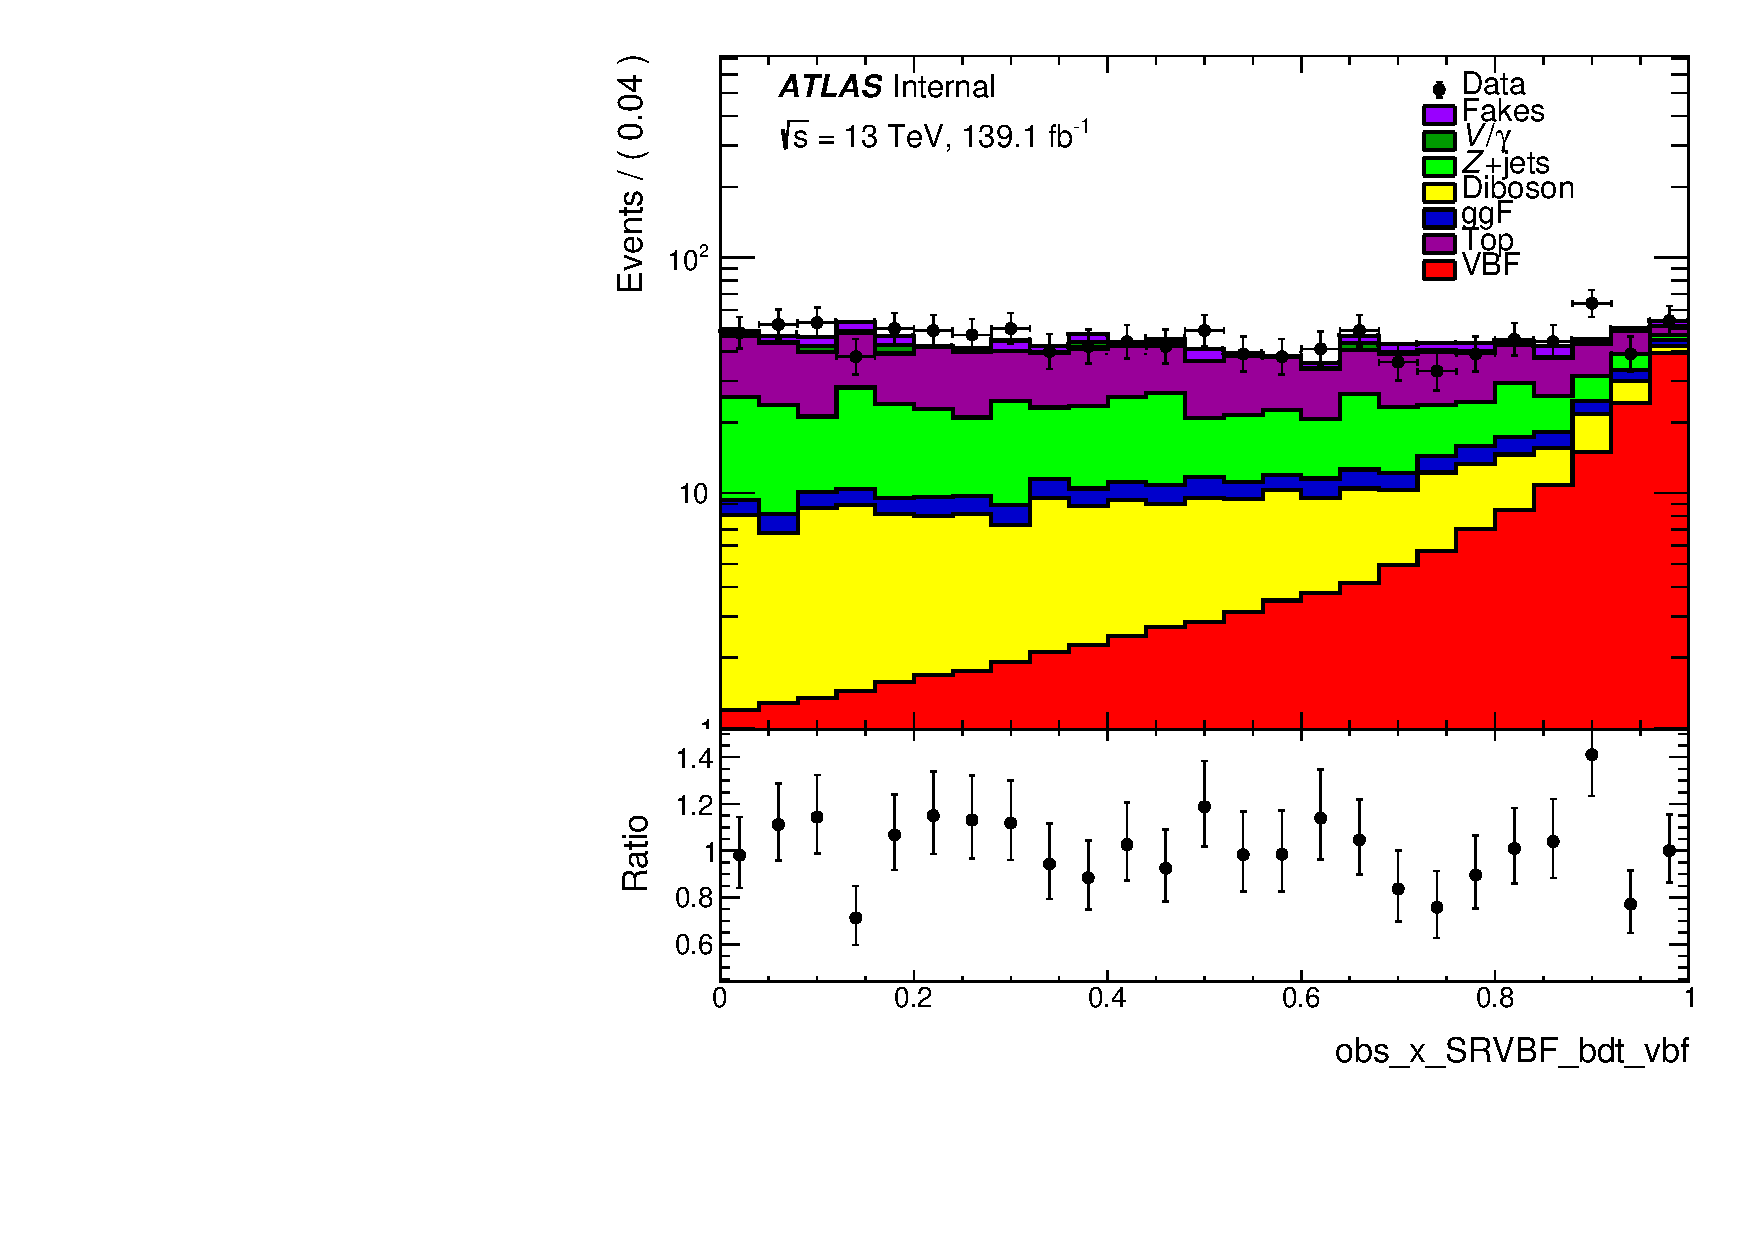
\includegraphics[width=0.3\textwidth]{Pictures/fitresults/SRVBF.pdf}
  }\hfill
  \subfloat[ggF 1 control region]{
      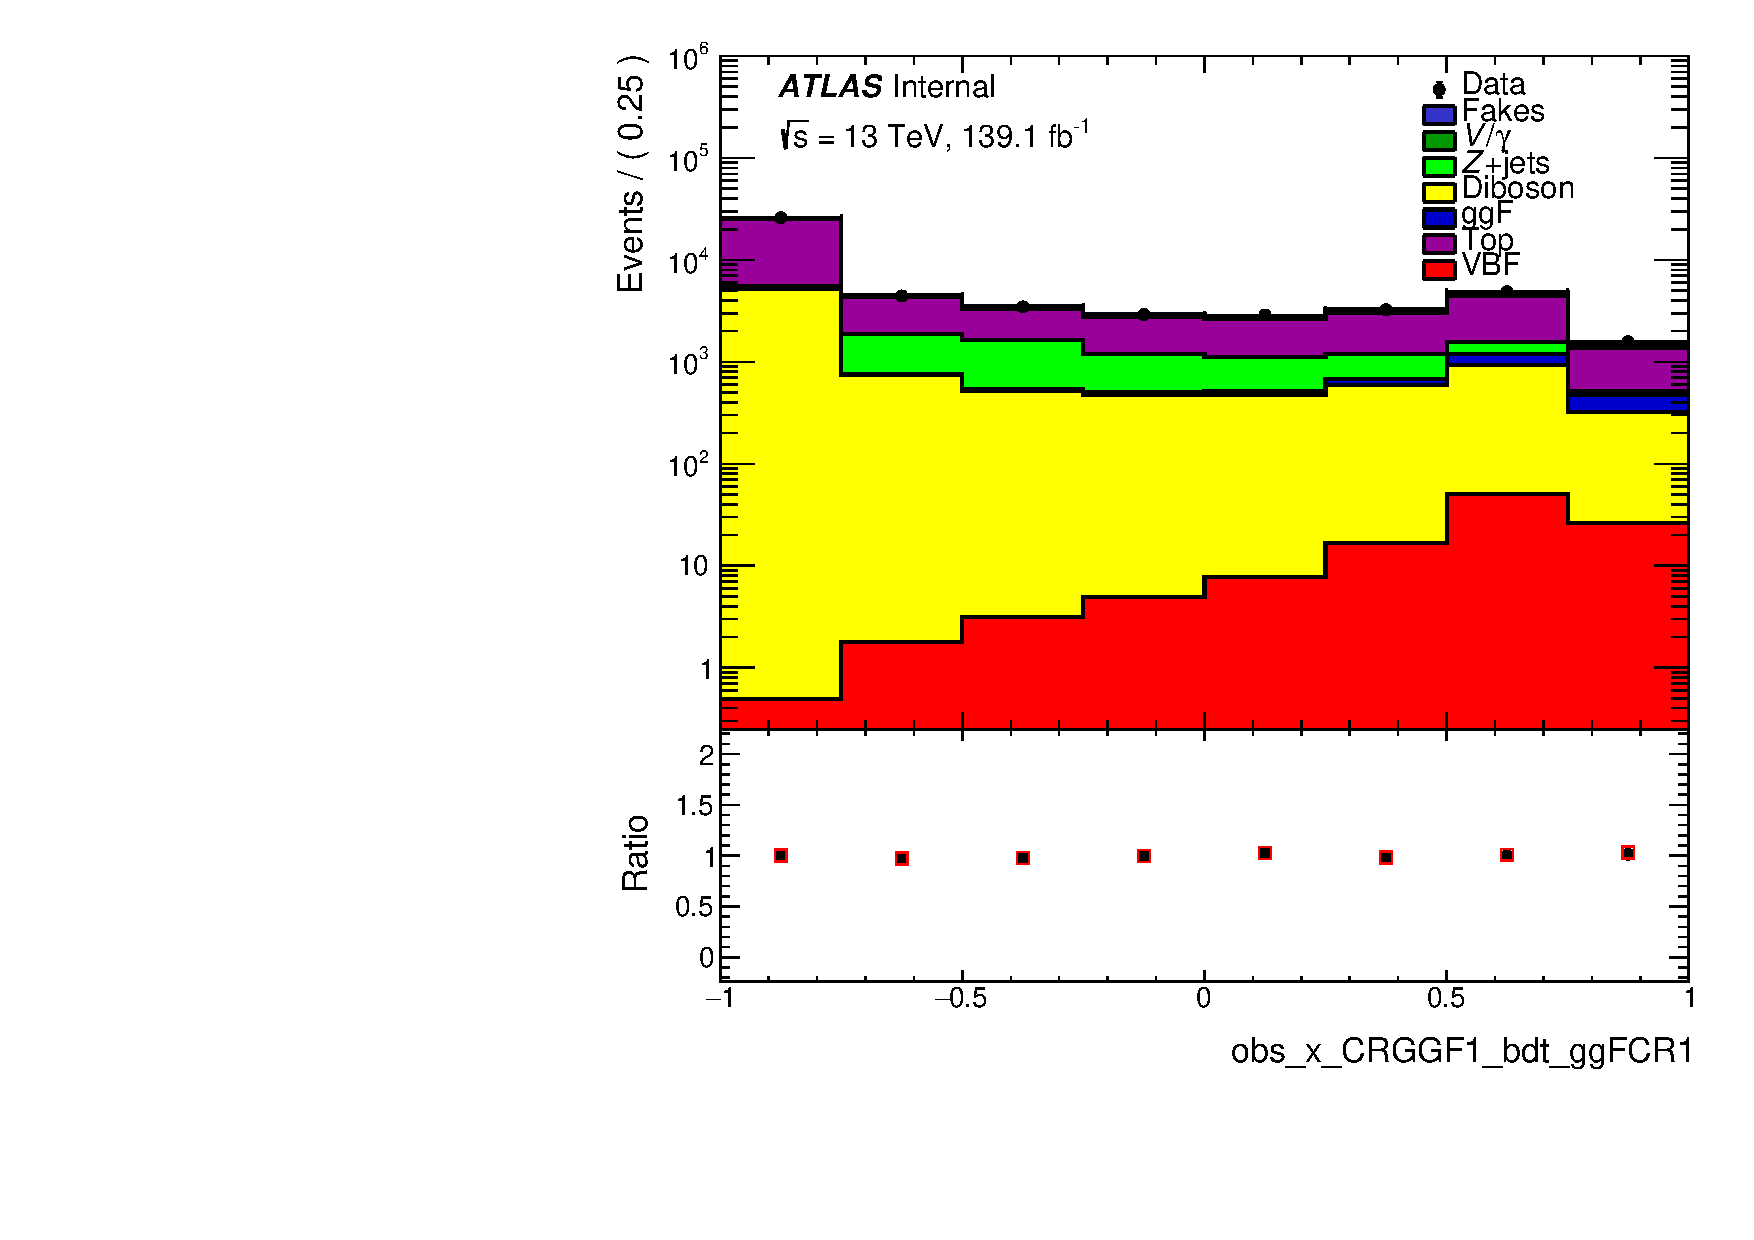
\includegraphics[width=0.3\textwidth]{Pictures/fitresults/CRGGF1.pdf}
  }\hfill
  \subfloat[ggF 2 control region]{
      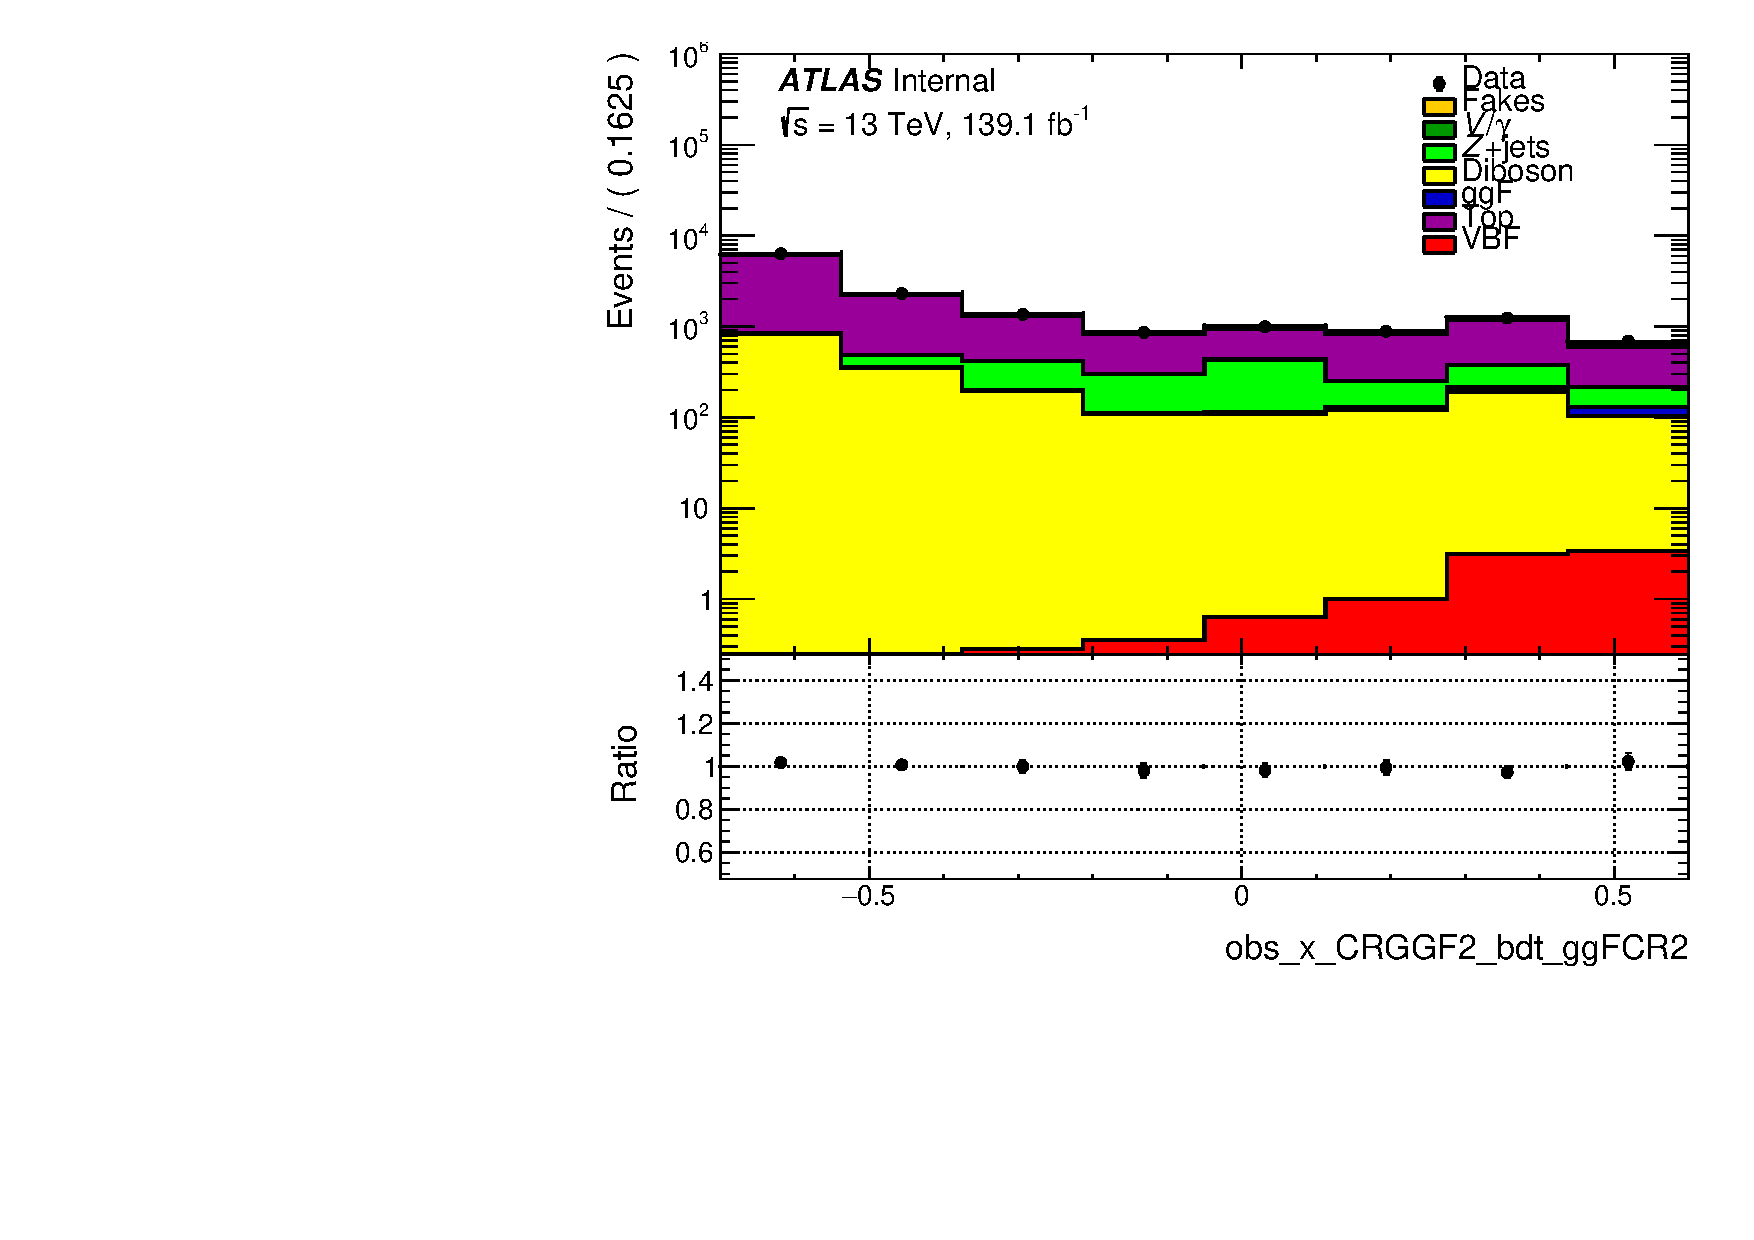
\includegraphics[width=0.3\textwidth]{Pictures/fitresults/CRGGF2.pdf}
  }\hfill
  \subfloat[ggF 3 control region]{
      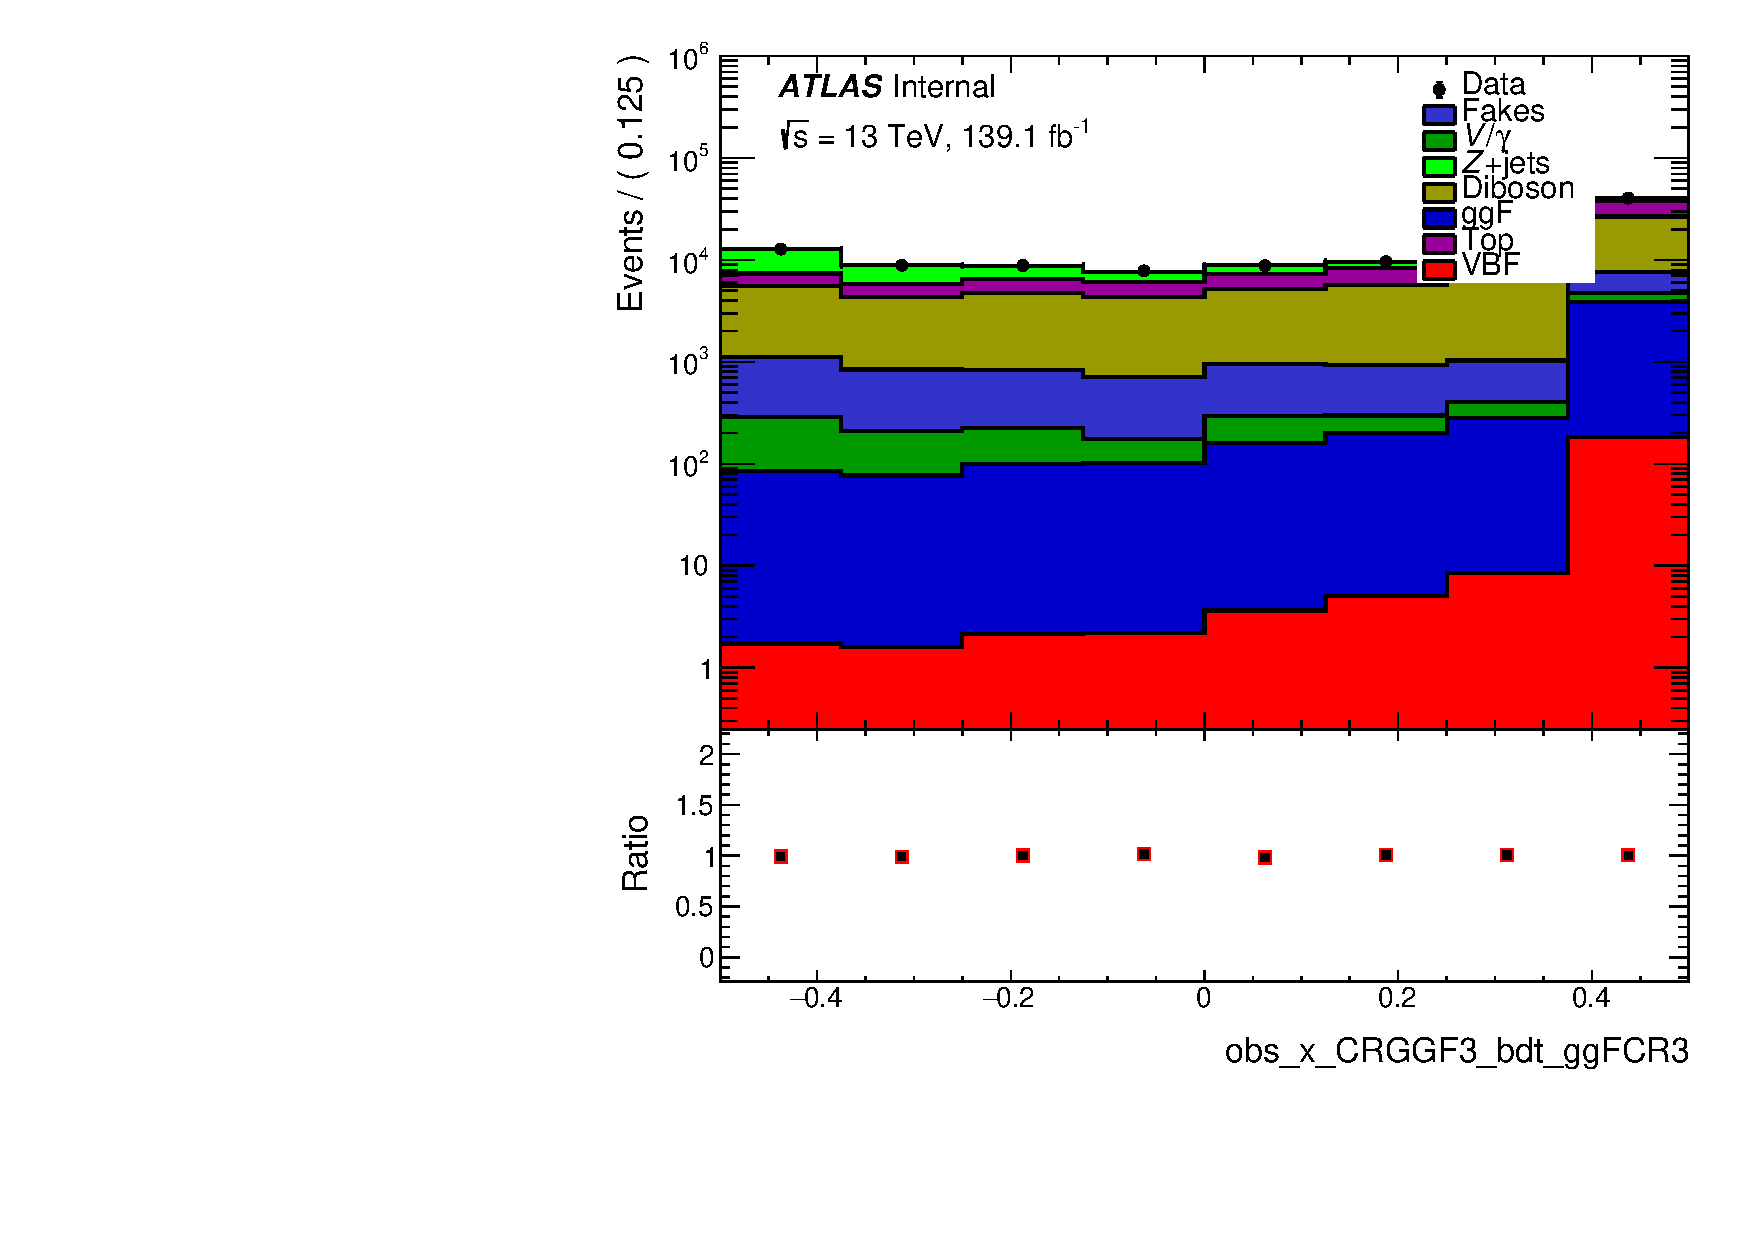
\includegraphics[width=0.3\textwidth]{Pictures/fitresults/CRGGF3.pdf}
  }\hfill
  \subfloat[$Z+$jets control region]{
      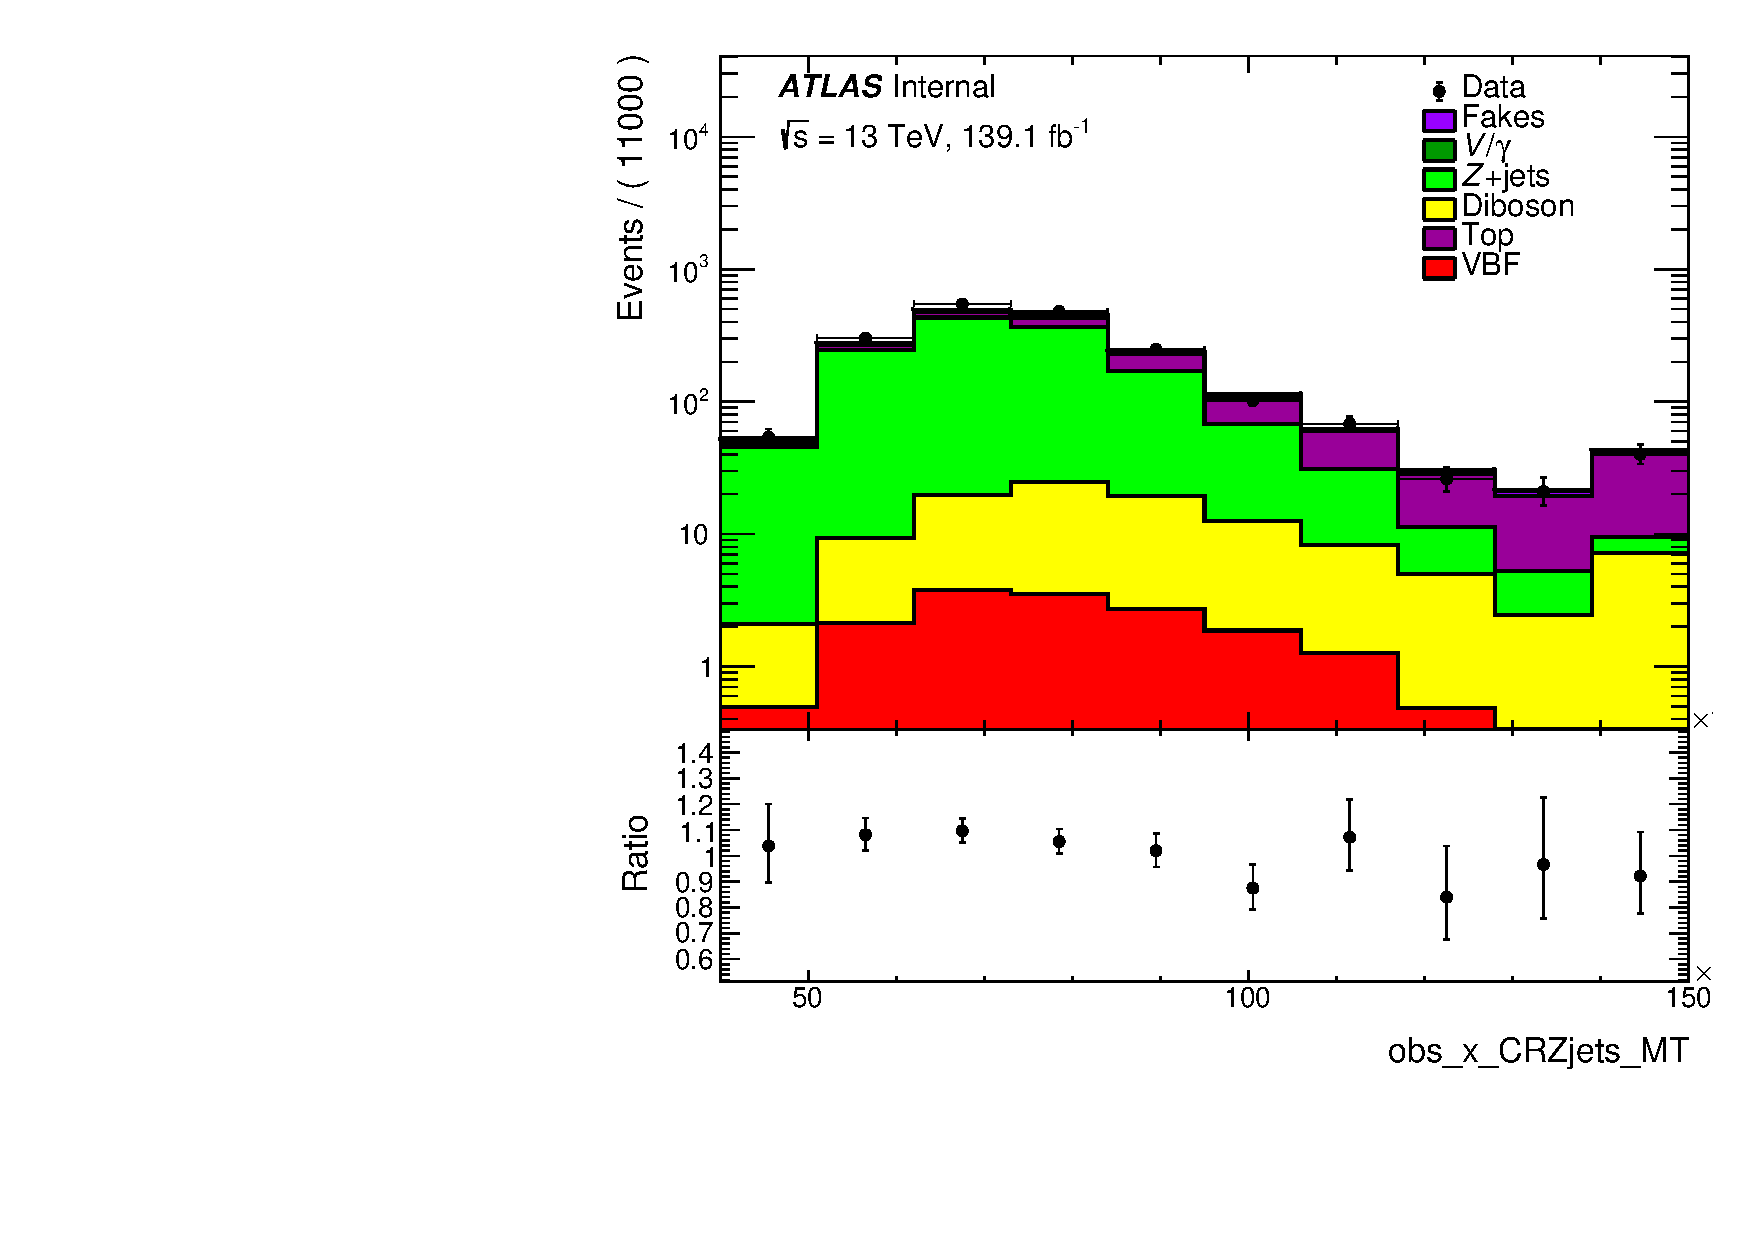
\includegraphics[width=0.3\textwidth]{Pictures/fitresults/CRZjets.pdf}
  }\hfill
  \subfloat[Top/$WW$ control region]{
      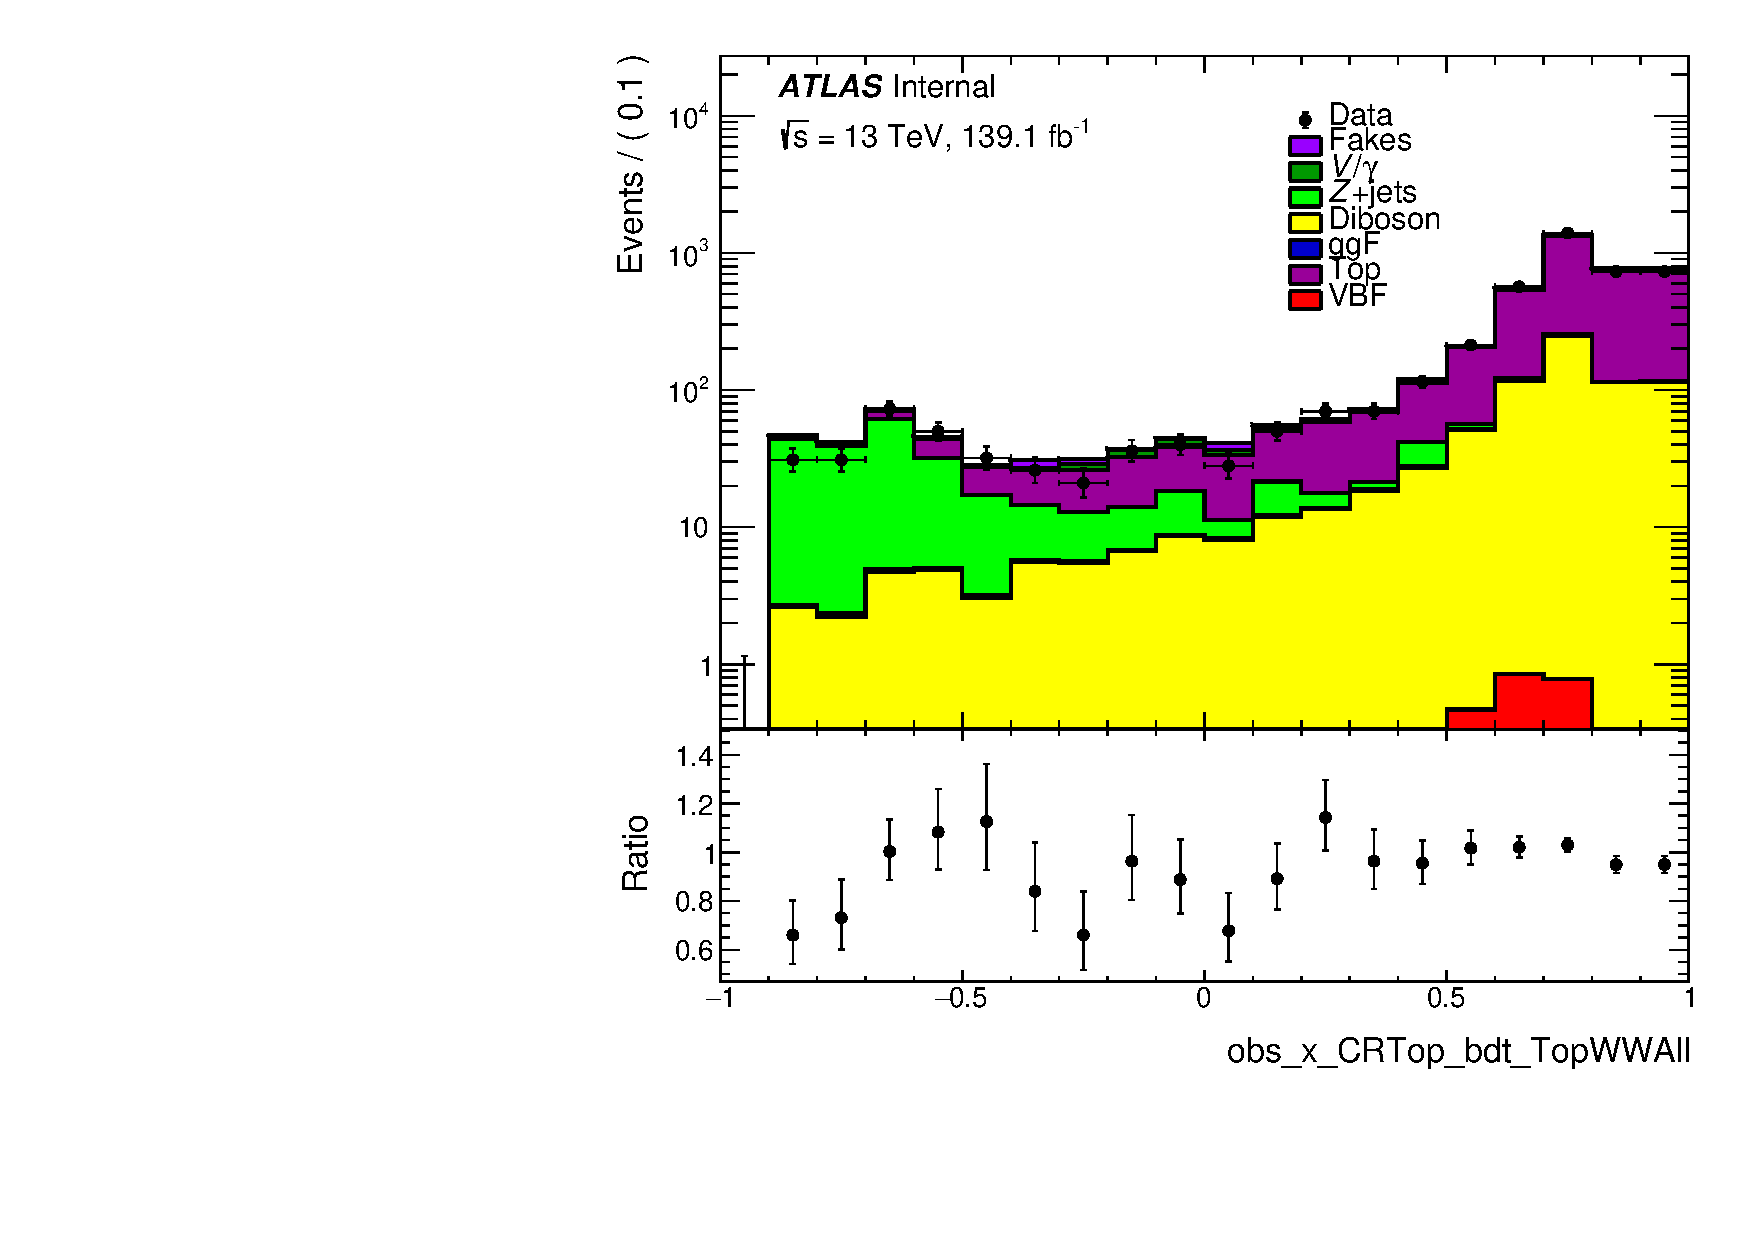
\includegraphics[width=0.3\textwidth]{Pictures/fitresults/CRTop.pdf}
  }%hfill
{\caption{Binned distributions for each signal and control region shown after stat-only fit where ratio between data and MC predictions is shown (black). Red points show VBF signal significance per bin.
\label{fig:fitresultsregions}}}
\end{figure}

The first fits performed use no nuisance parameters, only statistical uncertainties, to show both how the overall fit performs at its most basic level and to deduce the overall impact of adding systematics to the fit. The plot \ref{fig:correlations} shows correlations between floating parameters in the fit using a stat-only scheme where only the seven floating signal strength parameters are fit.

\begin{figure}[!h]
\centering
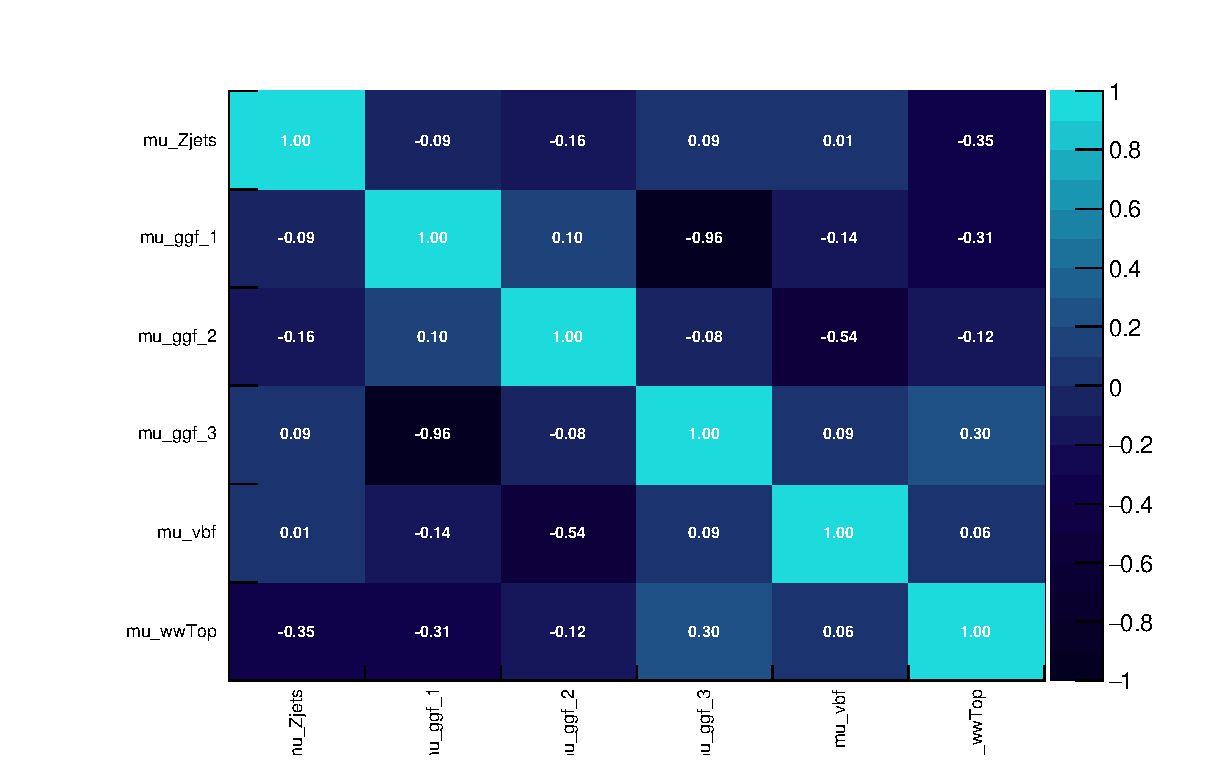
\includegraphics[width=0.45\textwidth]{Pictures/fitresults/correlation_stat.eps}
\caption{Correlations between floating parameters after a stat-only fit}
\label{fig:correlations}
\end{figure}

We can visualize and better understand these results through a 1D scan of our parameter of interest ($\mu_{\text{VBF}}$). Using the inputs and distributions of of our fit we can view the minimization of the total likelihood and and its width the see the impact of systematics and constraints from the other floating parameters. Plots \ref{fig:scan} shows fit results for $\mu_{\text{VBF}}$ if we use all systematics, only statistical uncertainties, and finally if were to leave only $\mu_{\text{VBF}}$ as a floating parameter and all other constant. These results demonstrate the substantial role systematics play in our analysis. We break down these impacts to assess which nuisance parameters have the greatest effects on each measured parameter so that we can find any that seem unduly high and find ways to control their effects through our event selection and fit techniques. The following plots \ref{fig:impacts} show the 40 largest impact parameters for each measured signal strength. These effects are derived post-fit which means that at the maximum of the likelihood each parameter is changed by $\pm 1\sigma$ individually. The measured effects of these changes are shown in blue on the plots and ranked in order of total combined positive and negative impact. 

\begin{figure}[!h]
\centering
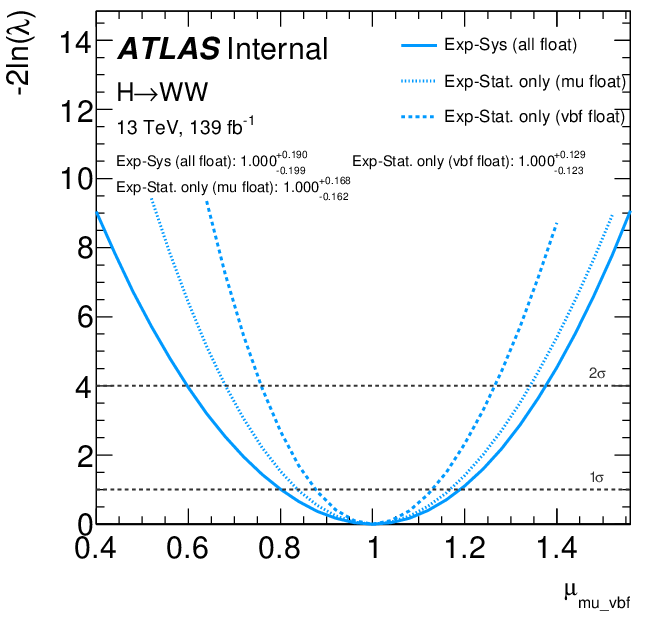
\includegraphics[width=0.45\textwidth]{Pictures/fitresults/afterfit.png}
\caption{Scan of $\mu_{\text{VBF}}$ negative log-likelihood using Asimov data and using only one floating parameter, all $\mu$ values floating, and all $\mu$ and NPs floating. \textcolor{red}{Will replace with unblinded/more final plot}}
\label{fig:scan}
\end{figure}

\begin{figure}[!h]
\centering
  \subfloat[$\mu_{\text{VBF}}$]{
      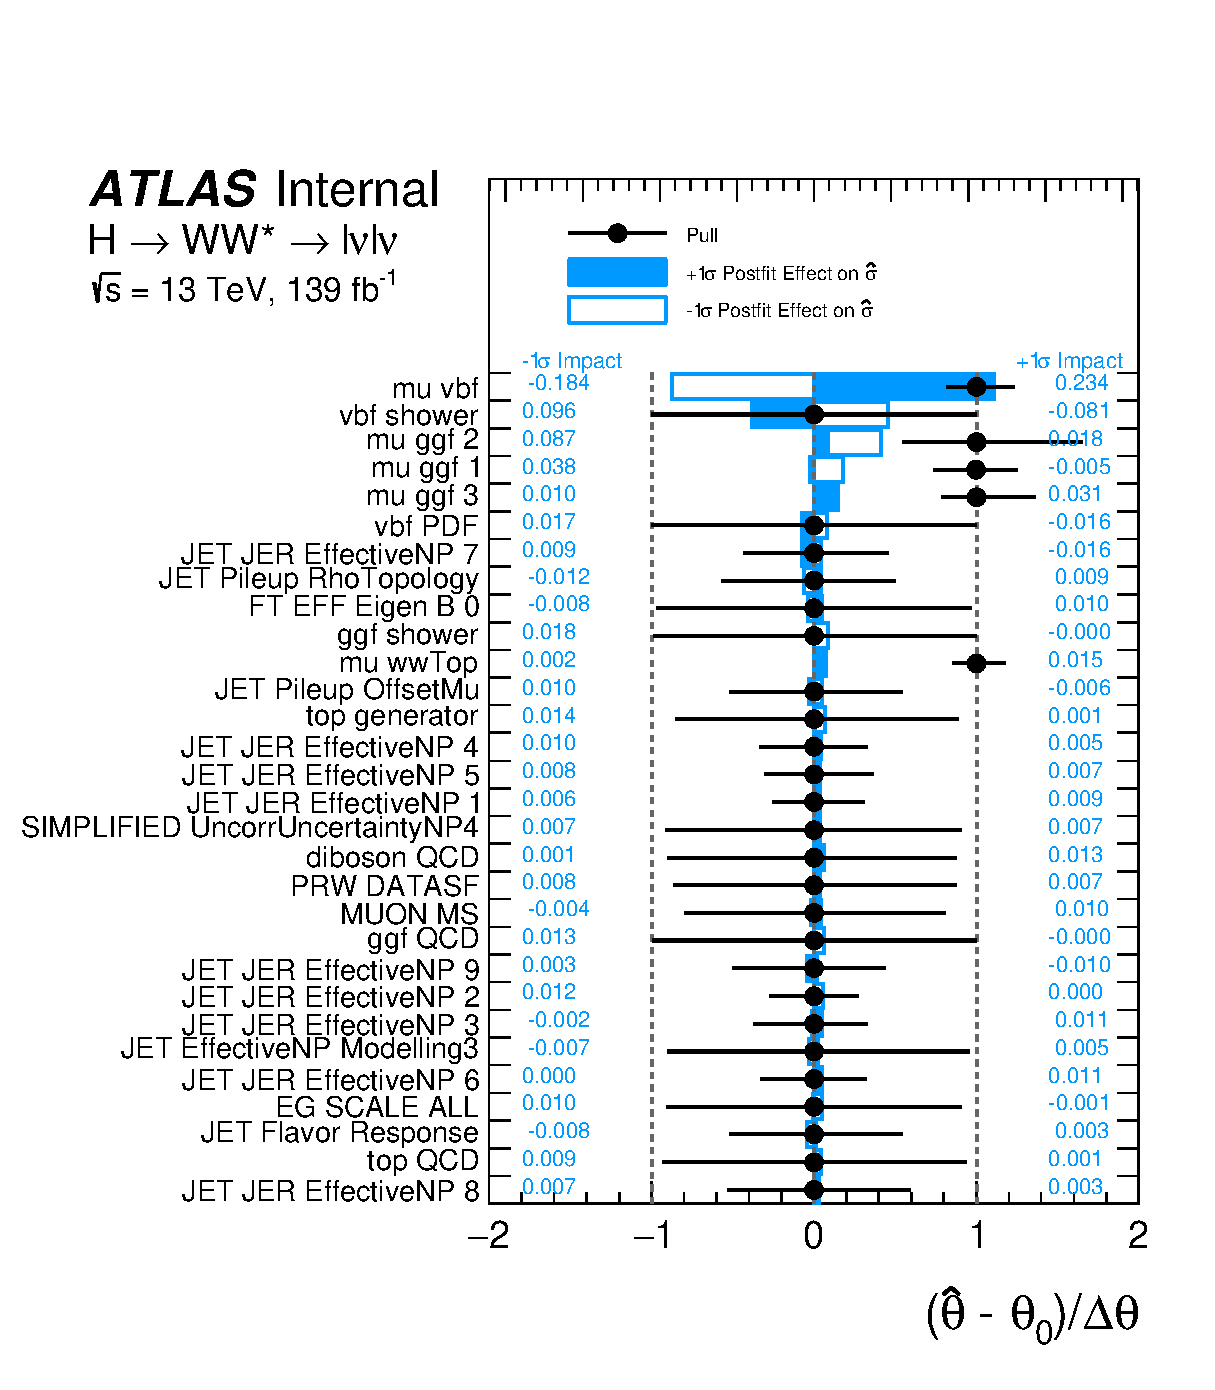
\includegraphics[width=0.3\textwidth]{Pictures/fitresults/impact_asimov_mu_vbf.eps}
  }\hfill
  \subfloat[$\mu_{\text{ggF}}$]{
      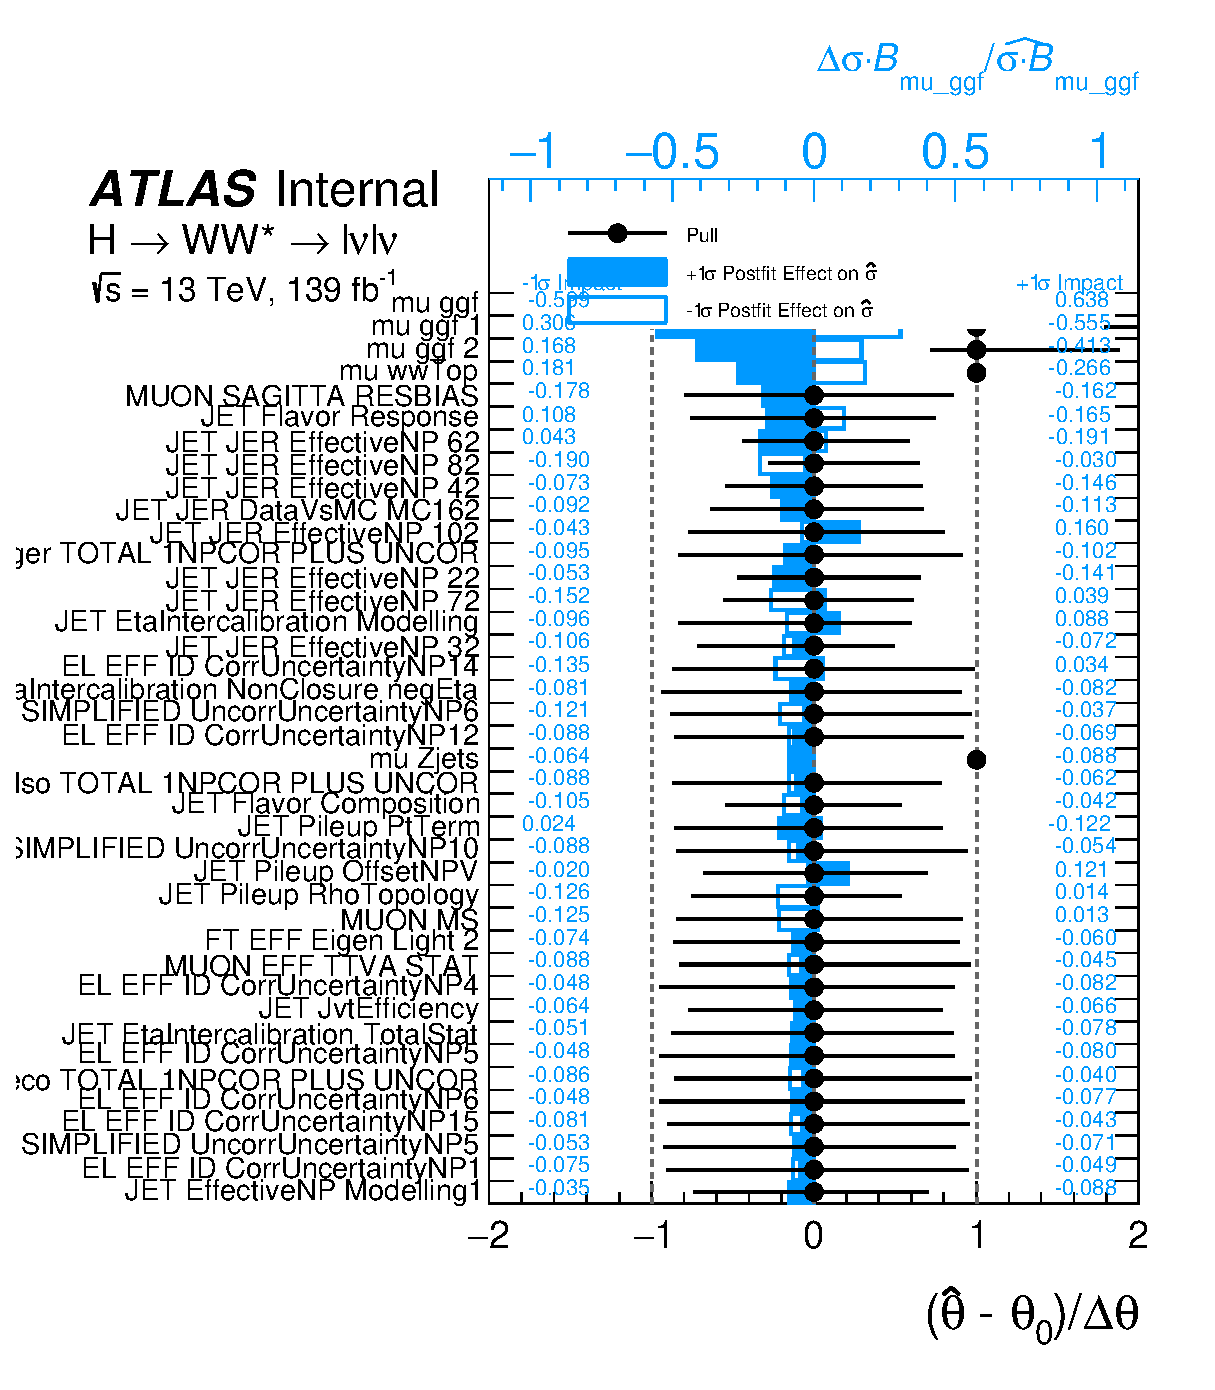
\includegraphics[width=0.3\textwidth]{Pictures/fitresults/impact_asimov_mu_ggf.eps}
  }\hfill
  \subfloat[$\mu_{\text{ggF1}}$]{
      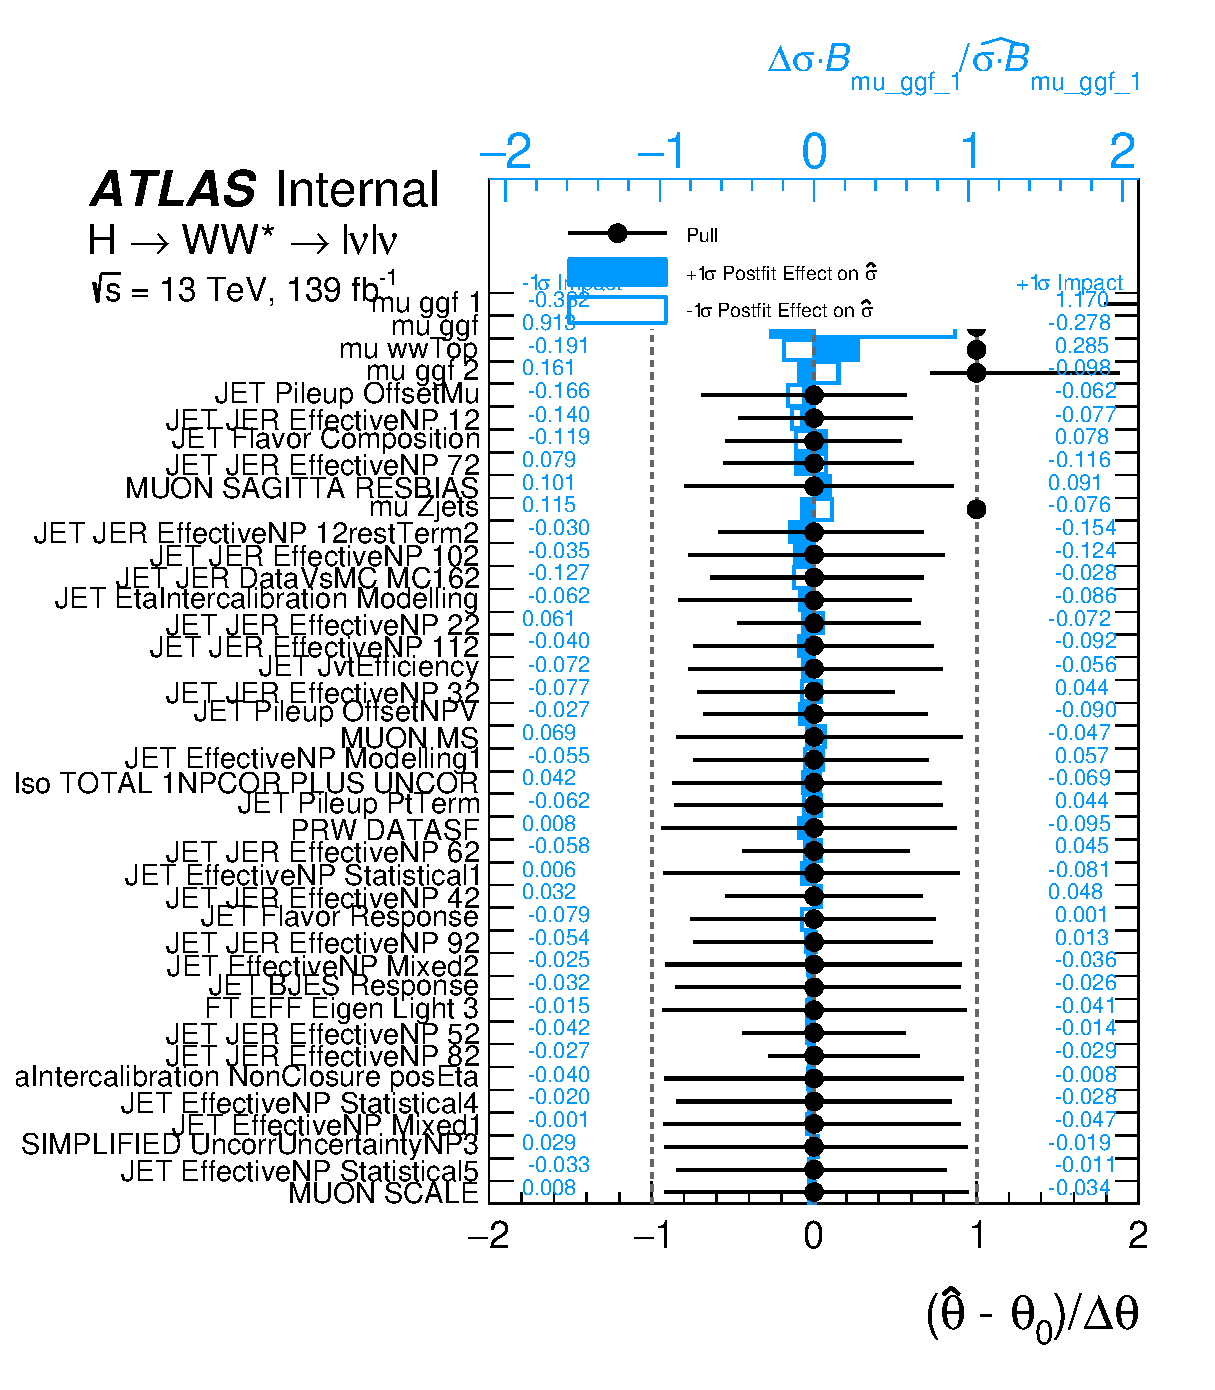
\includegraphics[width=0.3\textwidth]{Pictures/fitresults/impact_asimov_mu_ggf_1.eps}
  }\hfill
  \subfloat[$\mu_{\text{ggF2}}$]{
      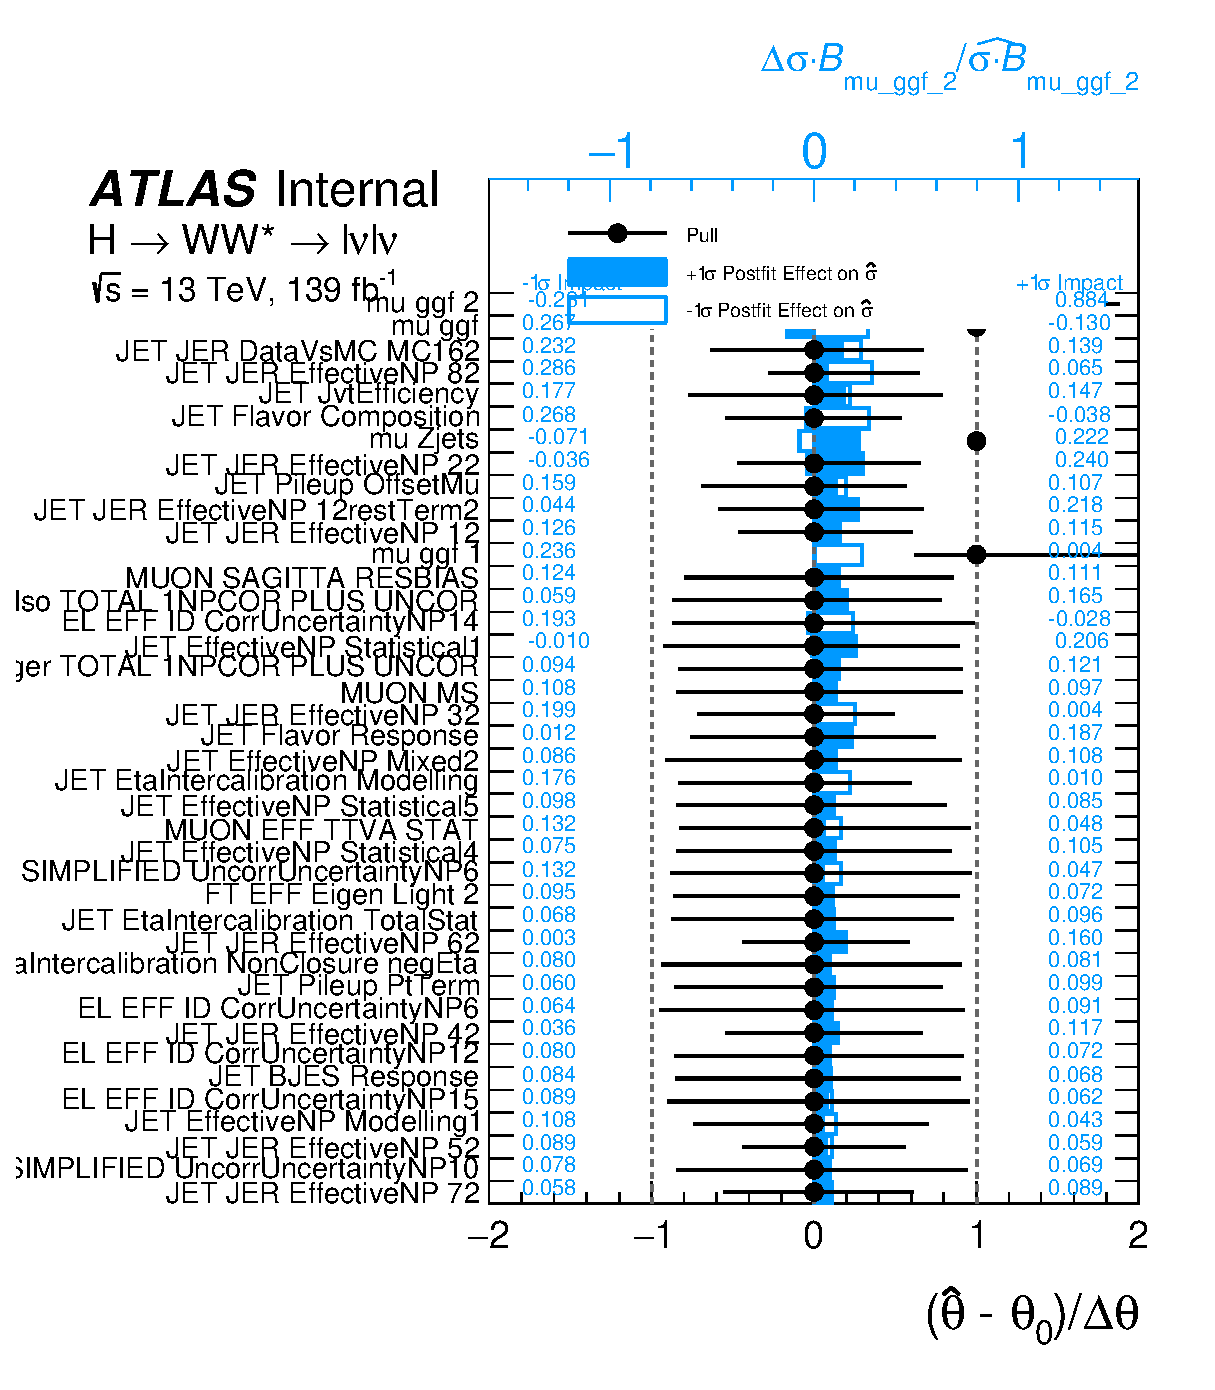
\includegraphics[width=0.3\textwidth]{Pictures/fitresults/impact_asimov_mu_ggf_2.eps}
  }\hfill
  \subfloat[$\mu_{\text{Top/}WW}$]{
      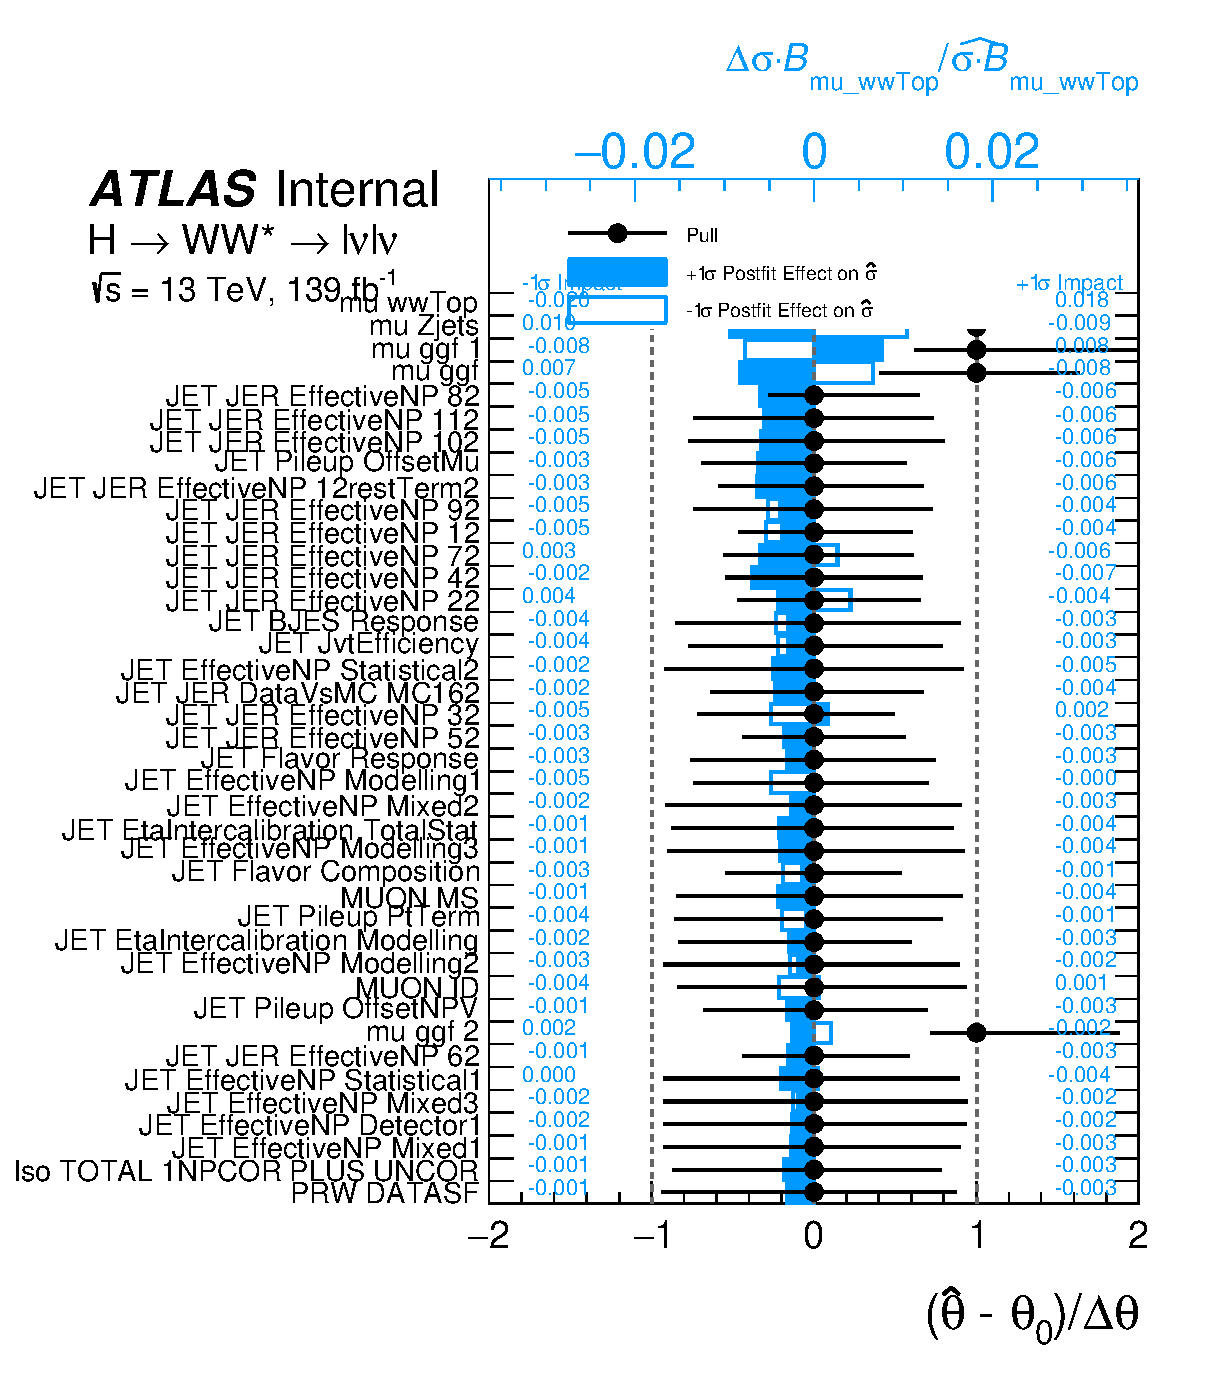
\includegraphics[width=0.3\textwidth]{Pictures/fitresults/impact_asimov_mu_wwTop.eps}
  }\hfill
  \subfloat[$\mu_{Z+\text{jets}}$]{
      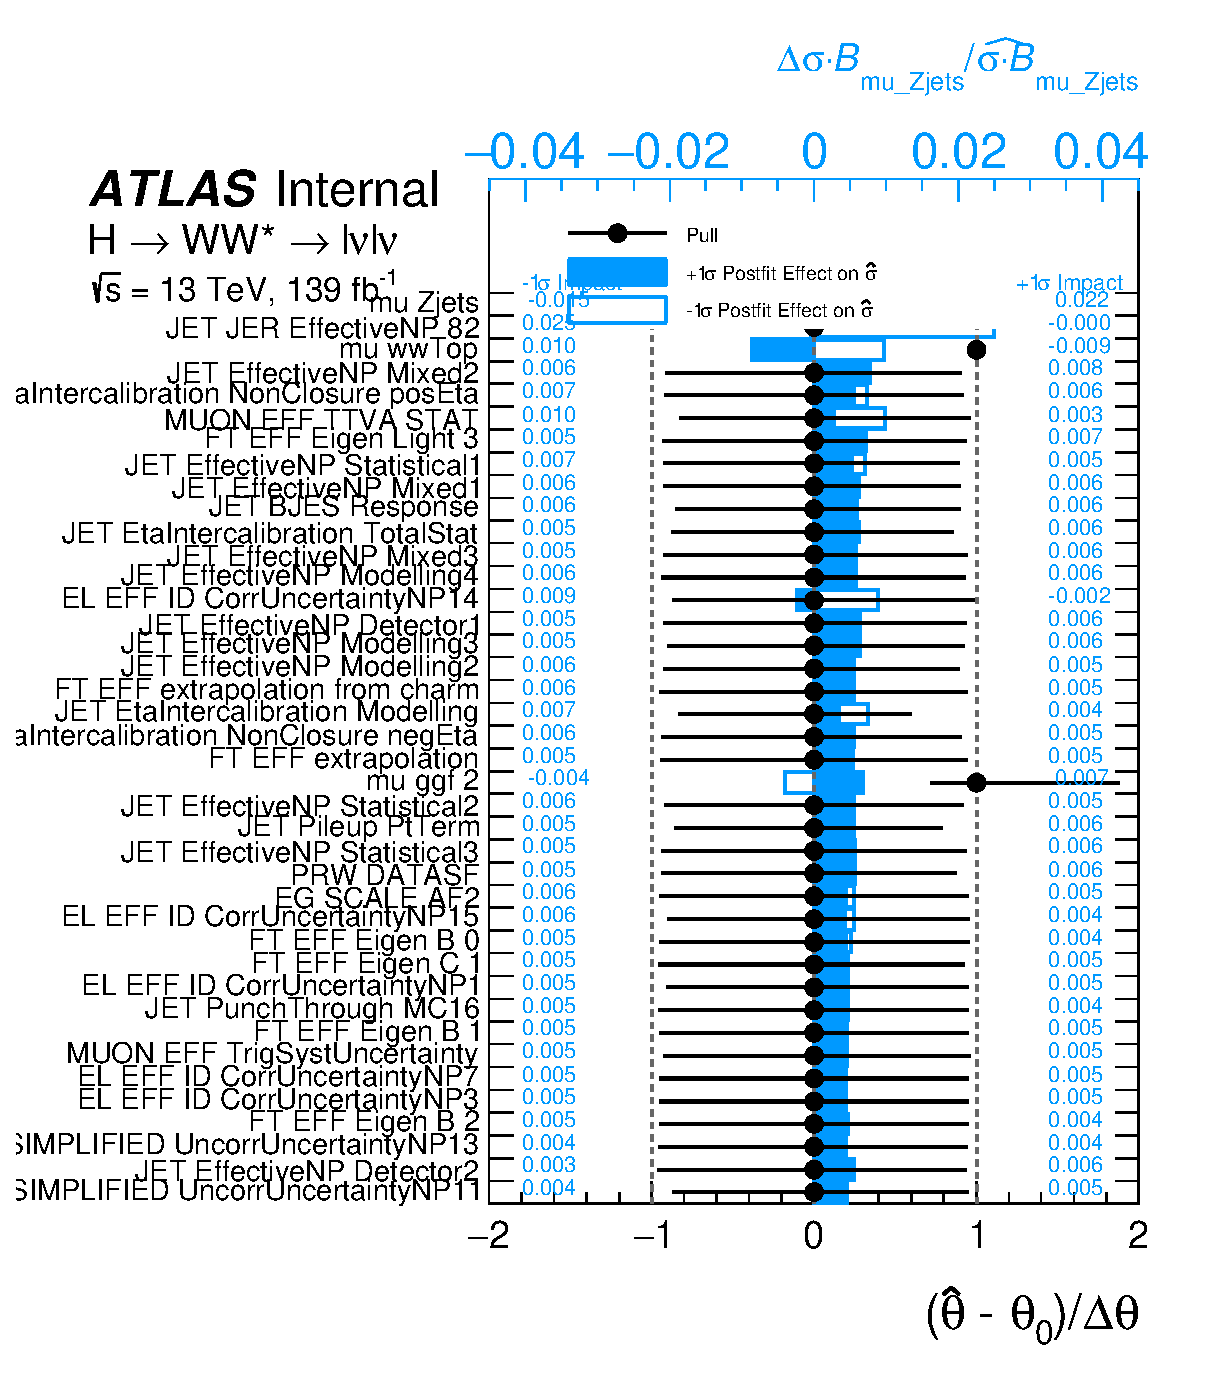
\includegraphics[width=0.3\textwidth]{Pictures/fitresults/impact_asimov_mu_Zjets.eps}
  }%hfill
{\caption{Impacts of top 40 most impactful nuisance parameters for each fit $\mu$ using Asimov data. \textcolor{red}{Will replace with unblinded, real plots}
\label{fig:impacts}}}
\end{figure}

The fit results shown in this thesis demonstrate the most recent calculations and developments from the VBF $H\rightarrow WW$ fiducial cross-section measurement but they are not yet complete. Additional theoretical uncertainties (as described in the previous chapter) need to be considered and evaluated. Final fit parameters may also continue to change before the analysis is published. 

\section{Fiducial and inclusive cross sections}
This analysis aims to measure the total VBF $H\rightarrow WW^*\rightarrow\ell\nu\ell\nu$ cross-section in both a particular fiducial region and in a more inclusive region in addition to the fiducial differential cross-section over a range of kinematic variables. In each case the measurement must be translated from one that only represents conditions in the ATLAS detector to values that can be understood with broad range of theoretical models. For fiducial measurements this can be done simply with a $C$ factor. First a fiducial region must be defined that is applicable to both reconstructed and purely theoretical (truth level) events. This fiducial region defines the conditions under which the cross-section is measured. The fiducial cross-section is defined:
\begin{equation}
\sigma_{\text{VBF}H\rightarrow WW^*\rightarrow\ell\nu\ell\nu}^{\text{fig}} = \frac{N_{\text{obs}}-N_{\text{bkg}}}{C\times\mathcal{L}}
\end{equation} 
where $\mathcal{L}$ is the integrated luminosity, and $N$ (obs,bkg) is the observed and estimated background number of events respectively. $N_{\text{bkg}}$ is the fit value of total background events from \ref{tab:postfityields}. $C$ is a factor that accounts for detector effects that would lower the overall cross-section like detector inefficiences and resolution effects. To minimize any necessary theoretical extrapolation, the fiducial phase space is defined as close to the reconstruction-level signal region as possible. The table \ref{tab:fiducial} lists all fiducial cuts that describe the phase space. These include requirements on lepton number, flavor, sign, and kinematics, missing energy, jet number, as well as other VBF specific requirements (OLV and CJV cuts). 
%Fiducial Volume
\begin{table}[!ht]
\centering
\begin{tabular}{|c|}
\hline
Fiducial Requirement \\
\hline
$|\eta(\ell)|<2.5$ \\
$p_T^{\text{lead}}>22$GeV \\
$p_T^{\text{sublead}}>15$GeV \\
$N_{\text{leptons}}\geq2$ \\
Leptons required to be opposite flavor and sign \\
$\Delta R(\ell,\ell) >$0.1 \\
$m_{\ell\ell}>10$GeV \\
$E_T^{\text{miss}}>$20GeV \\
$p_T$(jet)$>$30 GeV \\
$|\eta\text{(jet)}|<4.5$ \\ 
$N_{\text{jets}} \geq 2$ \\
$N_{b\text{-jet}} < 1$ \\
$m_{jj} >200$GeV \\
$\Delta Y_{jj}>2.1$ \\
$\Delta R(\ell,\text{jet})>0.4$ \\
OLV$=1$ \\
CJV$>20$GeV \\
\hline
\end{tabular}
\caption{Fiducial phase space definition}
\label{tab:fiducial}
\end{table}
These cuts represent the space within which both reconstruction-level and truth-level cross-sections are measured. Using yields extracted from the statistical fit and a $C$-factor we define with 
\begin{equation}
C = \frac{N_\text{fid}}{N_{\text{reco}}}
\end{equation}
where $N_\text{fid}$ is extacted from theoretical simulation. $Powheg+Pythia8$ are used to extract theoretical yields in the fiducial region. There are $436.62$ truth VBF Higgs events in the fiducial region. Using the fit yield from \ref{tab:postfityields} gives $C=2.63$

Using this value for $C$ and our observed number of events from data, we find a fiducial cross-section measurement:
\begin{equation}
\sigma_{fid,obs} = 3.12 \pm 0.624 \text{fb} 
\end{equation}
\textcolor{red}{This is stat-only}

The inclusive cross-section requires one additional acceptance correction factor $A$, which is estimated from theoretical calculations and extrapolates the fiducial cross section to a more inclusive phase space defined solely by a requirement for $N_{\text{jets}}\geq2$ where each jet has $p_T>30$GeV. This will be calculated from
\begin{equation}
\sigma_{VBF}^{\text{incl}} = \frac{\sigma_{VBF}^{\text{fid}}}{A}.
\end{equation}
The inclusive cross-section widens the applicable phase space of the measurement and provides another useful metric to compare data with expected Standard Model results. The $A$ factor is found through theoretical calculations which use VBFNLO to estimate VBF processes at next-to-leading order in QCD. The theoretical fiducial cross section is found to be $3.14$ fb and the inclusive VBF $H\rightarrow WW^*\rightarrow \ell\nu\ell\nu$ cross section is measured at 85.79 fb. The acceptance factor is therefore measured at $0.0366$. Using this factor we calculate an inclusive cross-section:
\begin{equation}
\sigma_{incl,obs} = 85.24 \text{fb}
\end{equation} 

\textcolor{red}{Include fit value, MC value and compare. P-value, sigma, error on $C$ and $A$}

\section{Differential cross-section measurements}
The differential cross-section measurement requires a more rigorous unfolding procedure than the total fiducial and inclusive cross-sections. Monte Carlo simulations processed in a pseudo-detector with all its expected inefficencies and limits (reconstruction-level) are compared to Monte Carlo simulations processed solely at the particle level (truth-level). The detector effects that influence reconstruction-level events are unfolded so that they match their truth-level counterparts. This reco-truth matching is a test that the unfolding process works as expected and does not bias results. After the analysis is unblinded, data will be unfolded using the same mechanisms to create a differential measurement that can be utilized beyond ATLAS. This analysis employs the iterative bayesian unfolding method\cite{bayesian} whose goal is to determine the probability that each bin $j$ in a reconstruction-level distribution corresponds to bin $i$ in a truth-level distribution. Using Bayes' theorem, this probability can be attained with knowledge of the true spectrum $T$ and the measured or reco-level spectrum $R$. We begin with Bayes' theorem: 
\begin{equation}
P(T_i|R)=\frac{P(R,T_i)P(T_i)}{\sum_{t} P(R,T_t)P(T_t)}
\end{equation}
where the demoninator is a normalization factor, $P(R,T_i)$ represents the likelihood and $P(T_i)$ the prior. The prior here is vague and so we begin with the assumption that $P(T_i)$ is constant. Hence the most probable spectrum for $T$ maximizes the likelihood. If we observe $n$ reco-level events, we can assign the probability of their true distributions through
\begin{equation}
\hat{n}(T_i)=n(R)\prod P(T_i|R).
\end{equation}
We then use resultant possibilities in the Bayes formula to evaluate $P(T_i|R_j)$. These values constitute the smearing matrix $M$. This matrix can then be used in turn to estimate the truth-level events in each bin of a distribution with
\begin{equation}
\hat{n}(T_i)=\frac{1}{\epsilon_i}\sum_{j=1}^{n_R} n(R_j)\prod P(T_i|R_j).
\end{equation}
where $\epsilon$ is the inefficiency, or ratio of events that pass both truth and reco-level selection by those that pass only truth. Finally the truth can be determined by the reconstructed bin-by-bin yields through
\begin{equation}
n(T_i)=\sum_j M_{ij} \prod n(R_j).
\end{equation}
The migration matrix thus directly maps reco-level distributions to truth-level. In order to calculate this matrix iteratively we first allow $P(T_i)$ to be a constant distribution, say $1/n_T$, which gives an expected number of truth events $n_0(C_i)=P_0(C_i)\prod n_R$. Next, calculate $\hat{n}(C)$ using the efficiency equation, and finally use $\chi^2$ to compare $\hat{n}(C)$ and $n_0(C)$. In the next iteration, $n_0$ is replaced by $\hat{n}$ and $P_0$ by $\hat{P}$ ($\hat{P(C_i)}=\hat{n}(C_i)/\hat{N_{true}}$) and the procedure continues until $\chi^2$ falls below a set threshold. 

While the final unfolding results fall beyond the scope of thesis, results for four kinematic variables are shown here. 
%ents. The figures below demonstrate that truth distribution (blue) and unfolded truth distributions (black) perfectly match as expected. Reco-level distributions are similarly shown, though these clearly differ from truth distributions. 

%\begin{figure}[!h]
%\centering
%\centering
%  \subfloat[$p^T_H$]{
%      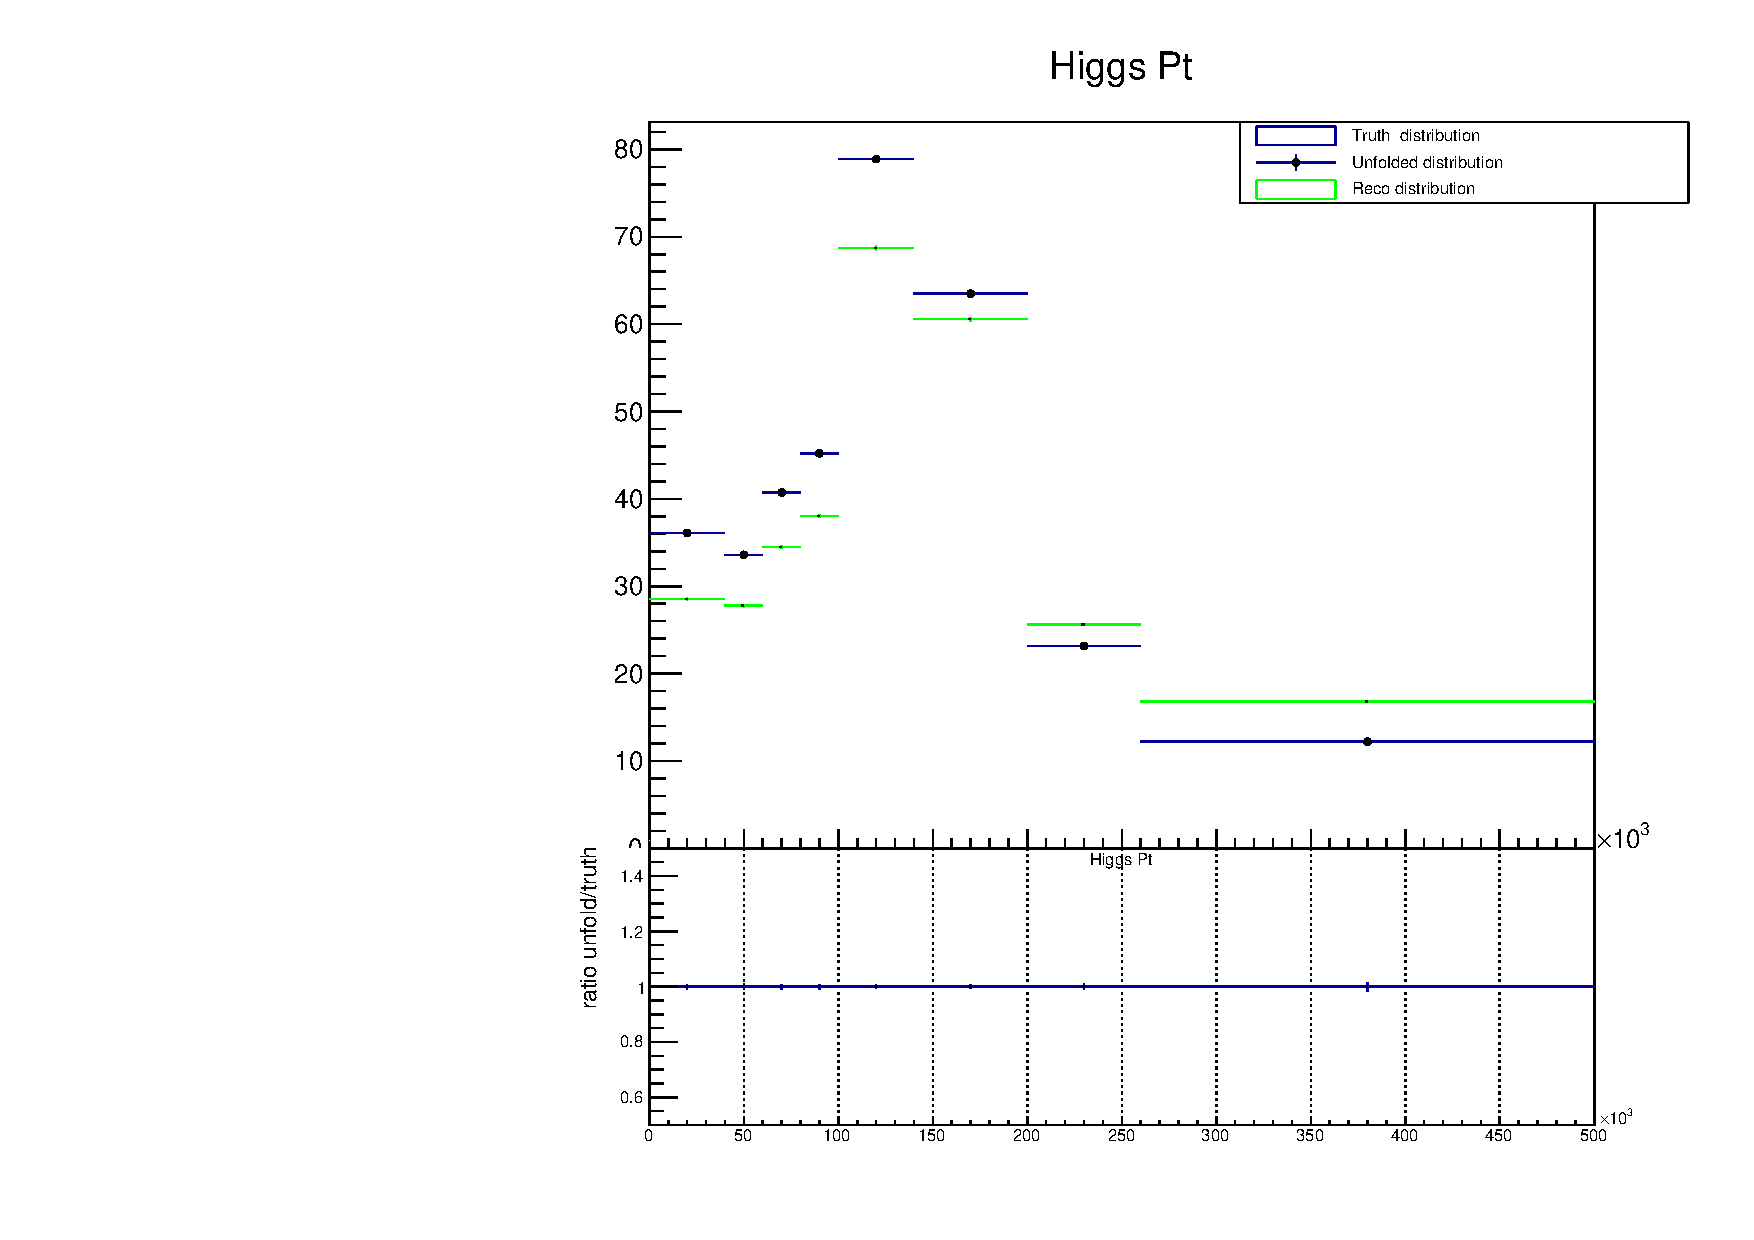
\includegraphics[width=.4\textwidth]{Pictures/unfolding/validation/higgs_pt_validation.pdf}
%  }\hfill
%  \subfloat[$m_T^{\ell\ell}$]{
%      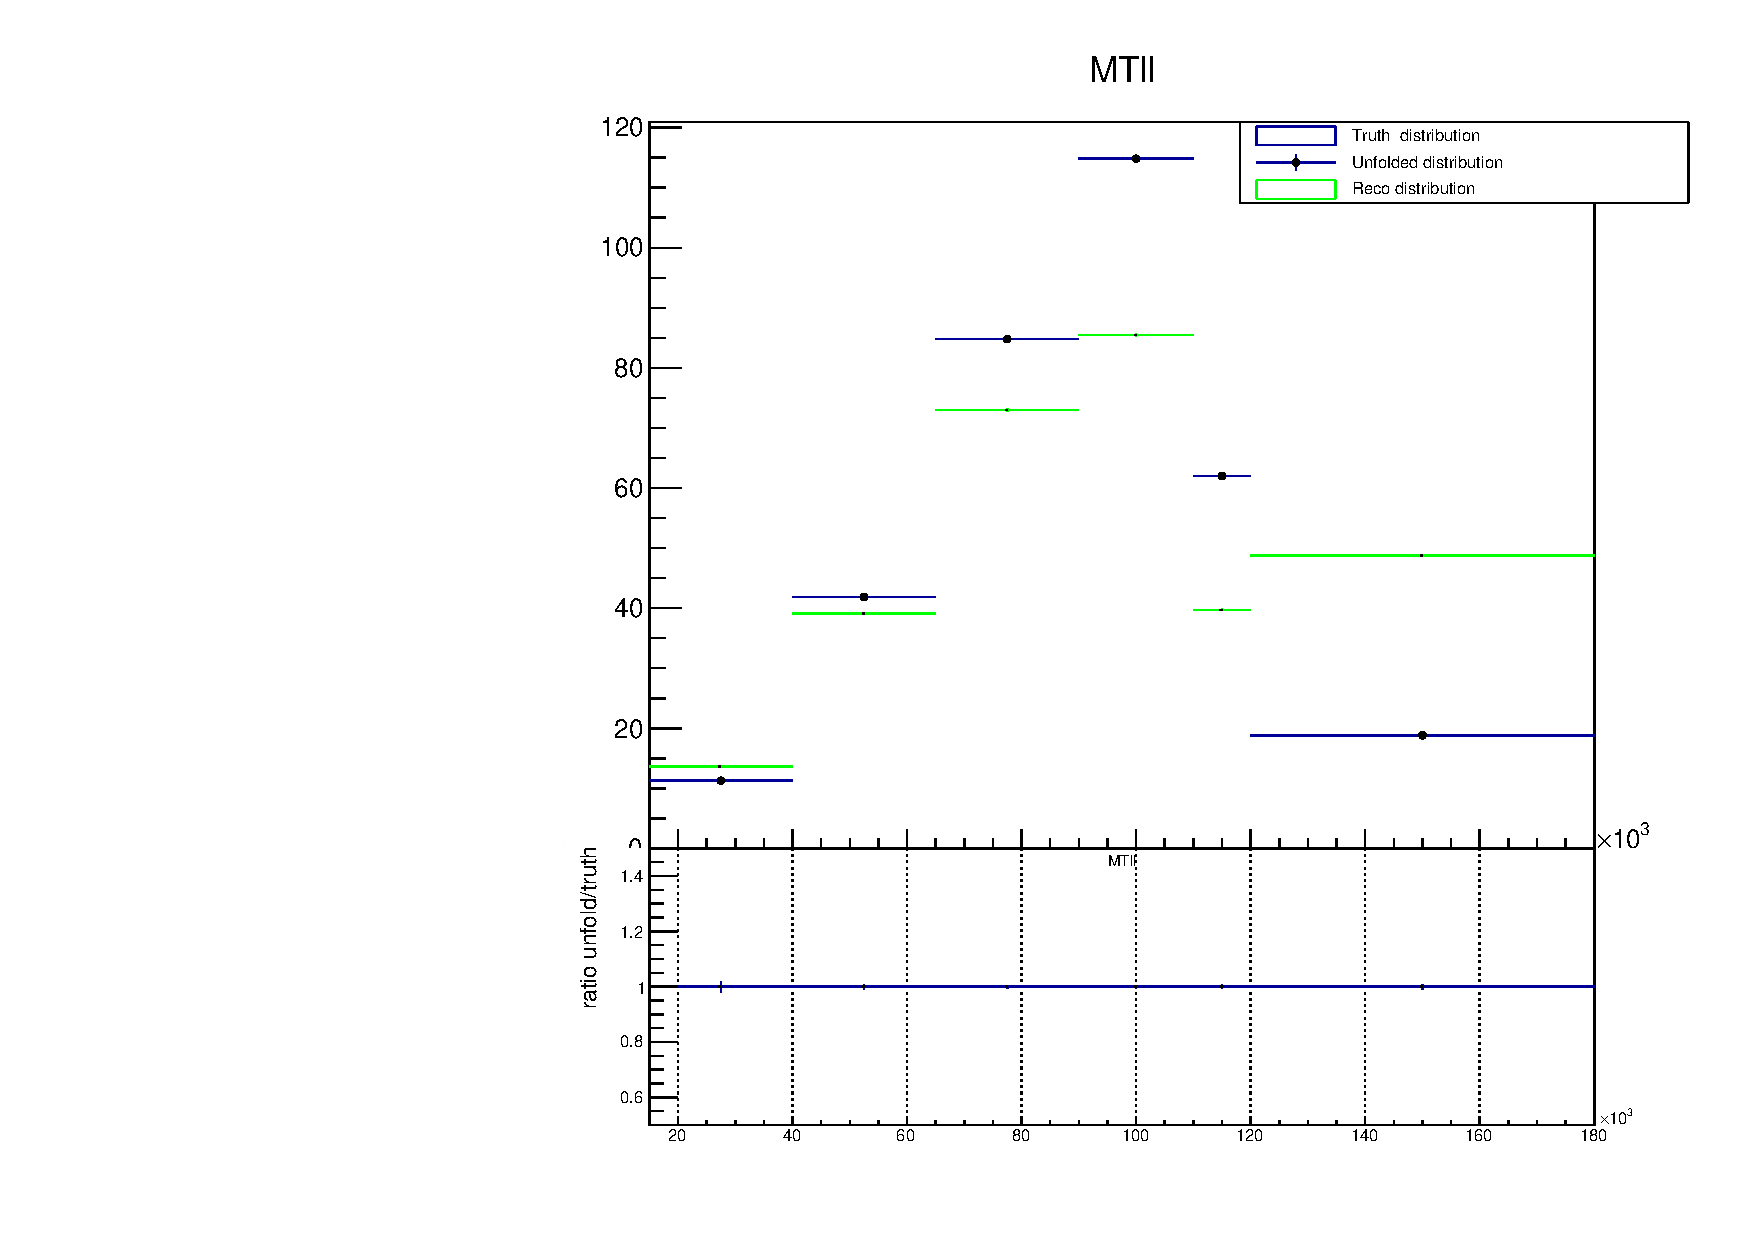
\includegraphics[width=.4\textwidth]{Pictures/unfolding/validation/MTll_validation.pdf}
%  }\hfill
%  \subfloat[$\Delta Y_{\ell\ell}$]{
%      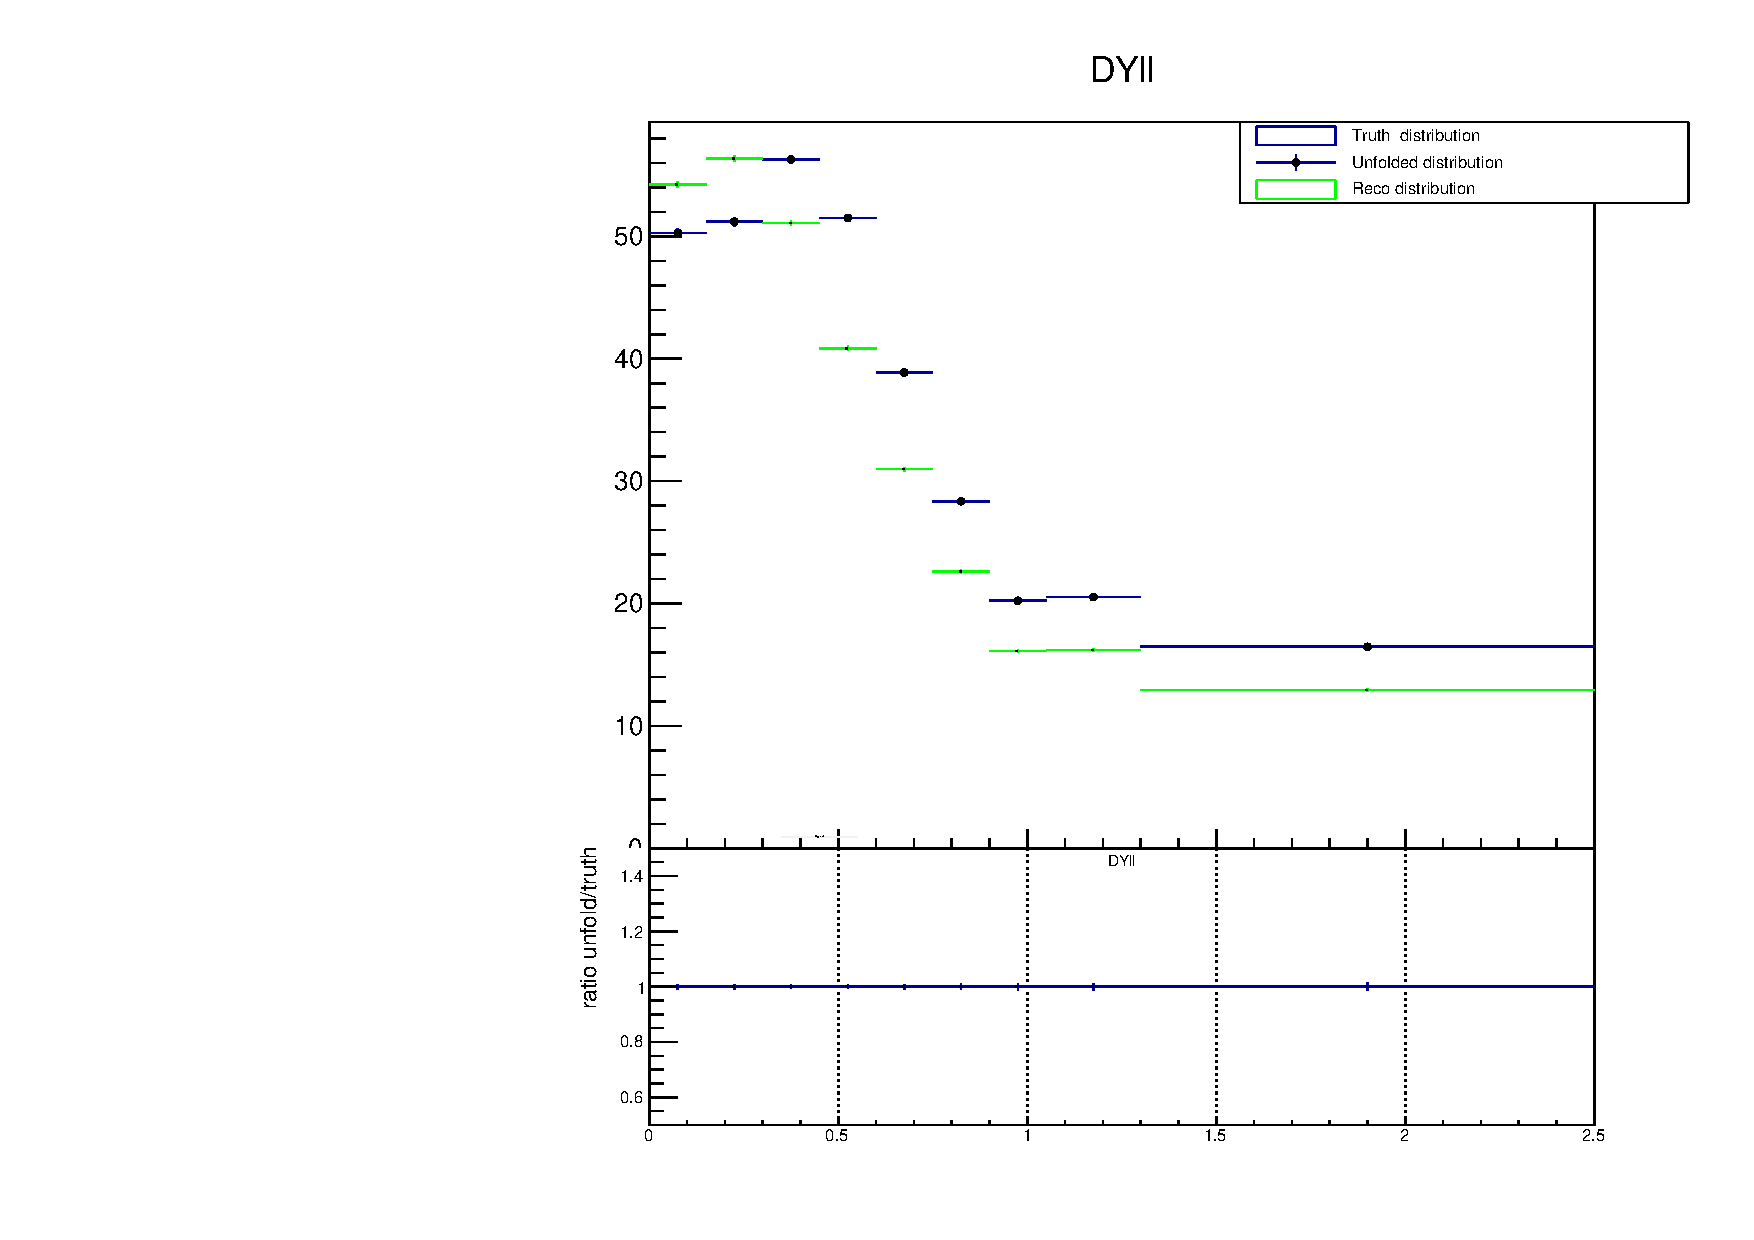
\includegraphics[width=.4\textwidth]{Pictures/unfolding/validation/DYll_validation.pdf}
%  }\hfill
%  \subfloat[$m_{jj}$]{
%      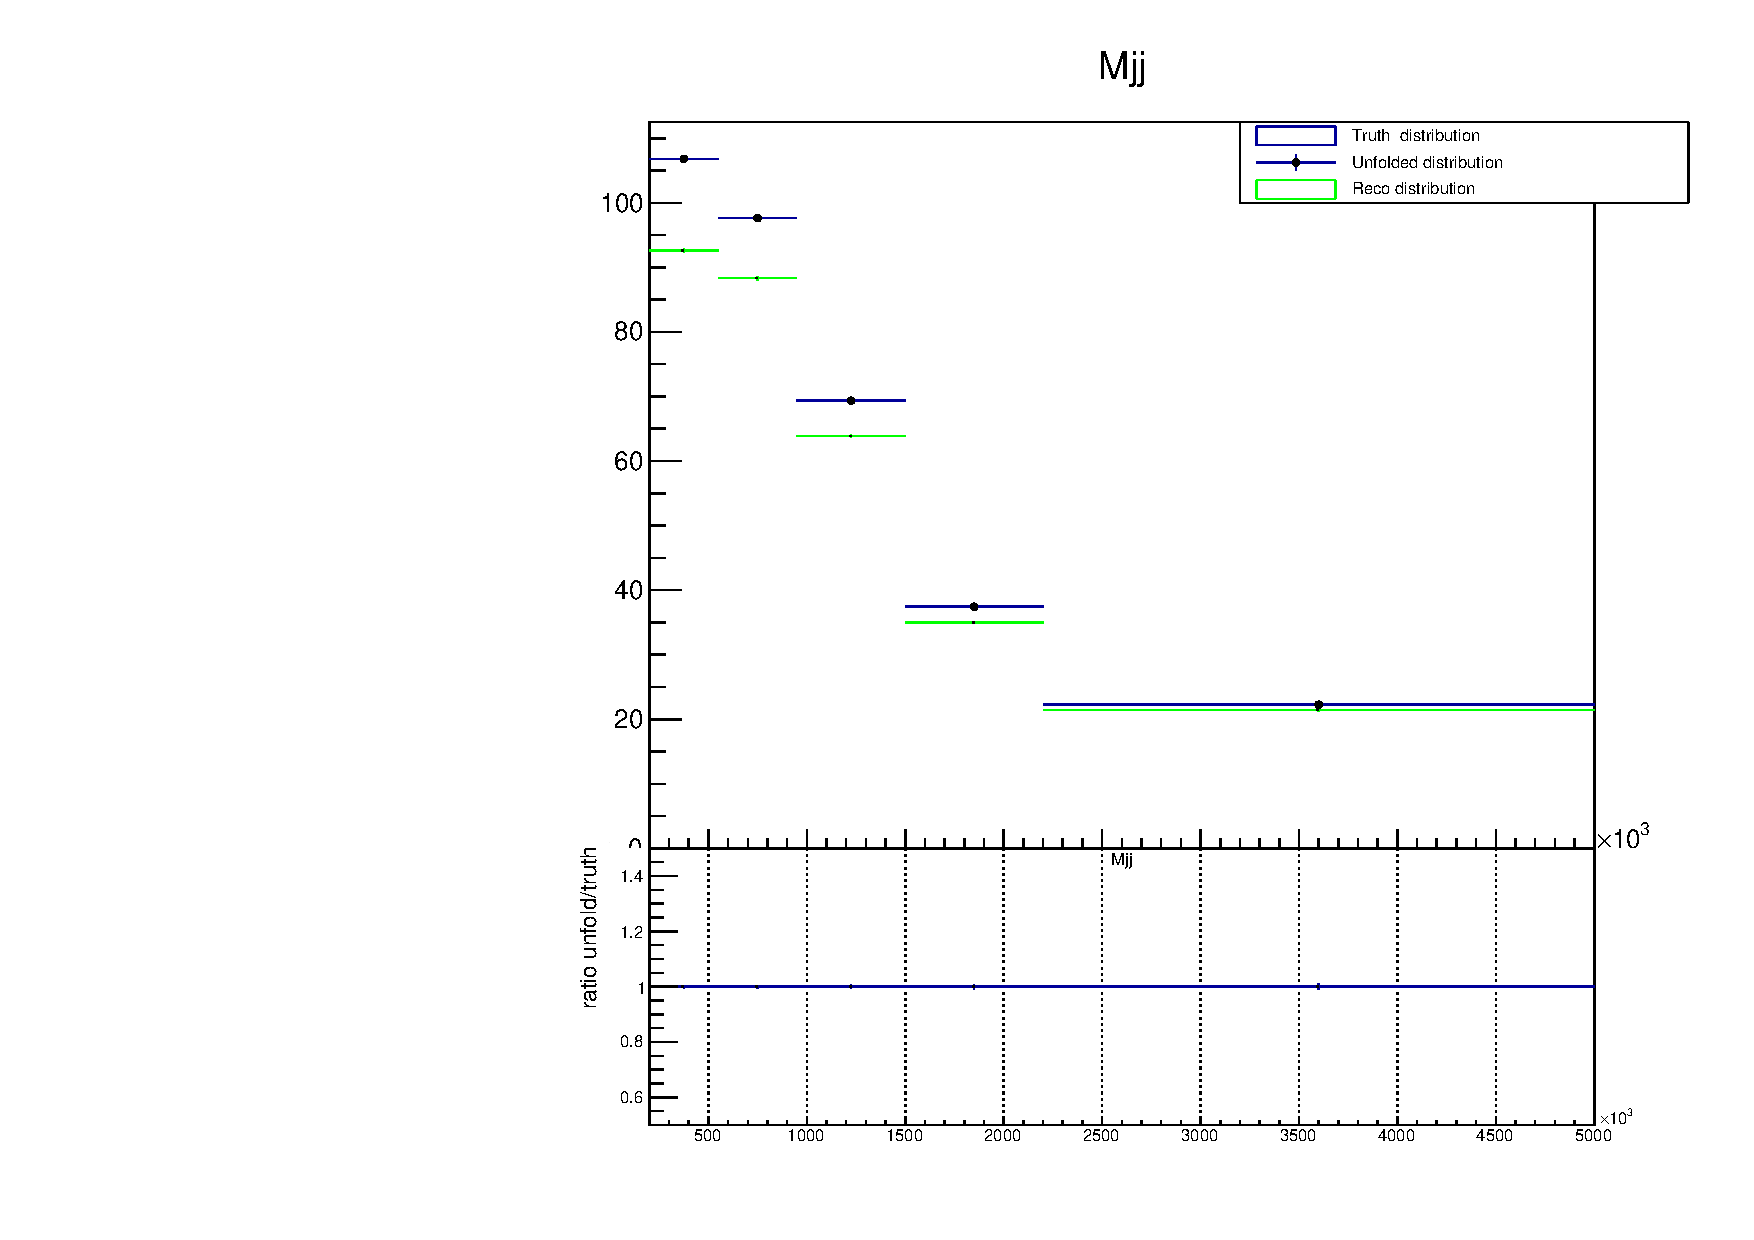
\includegraphics[width=.4\textwidth]{Pictures/unfolding/validation/Mjj_validation.pdf}
%  }%hfill
%\caption{\label{fig:unfoldingvalidation}Validation for unfolding mechanism, truth (blue) and unfolded truth distributions (black) overlap while reconstruction level distributions (green) fall separately. Distributions shown for $p^T_H$, $m_T^{\ell\ell}$, $\Delta Y_{\ell\ell}$ and $m_{jj}$**}
%\end{figure}

We use reconstruction-level Monte Carlo events and their truth counterparts to calculate migration matrices for each differential observable through the iterative Bayesian unfolding process. Four example migration matrices are shown in \ref{fig:unfoldingmatrices}. 

\begin{figure}[!h]
\centering
  \subfloat[$p^T_H$]{
      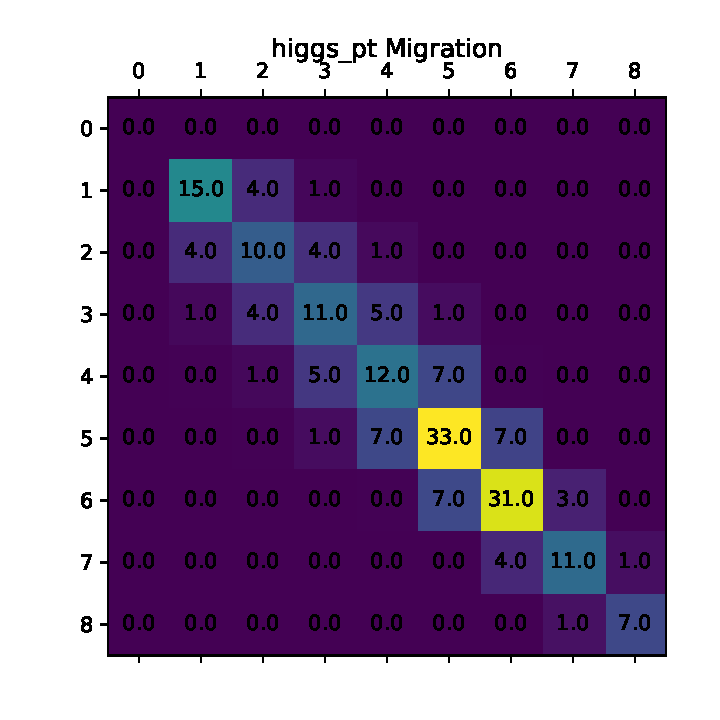
\includegraphics[width=.4\textwidth]{Pictures/unfolding/response_matrices/higgs_pt_migrations.pdf}
  }\hfill
  \subfloat[$m_T^{\ell\ell}$]{
      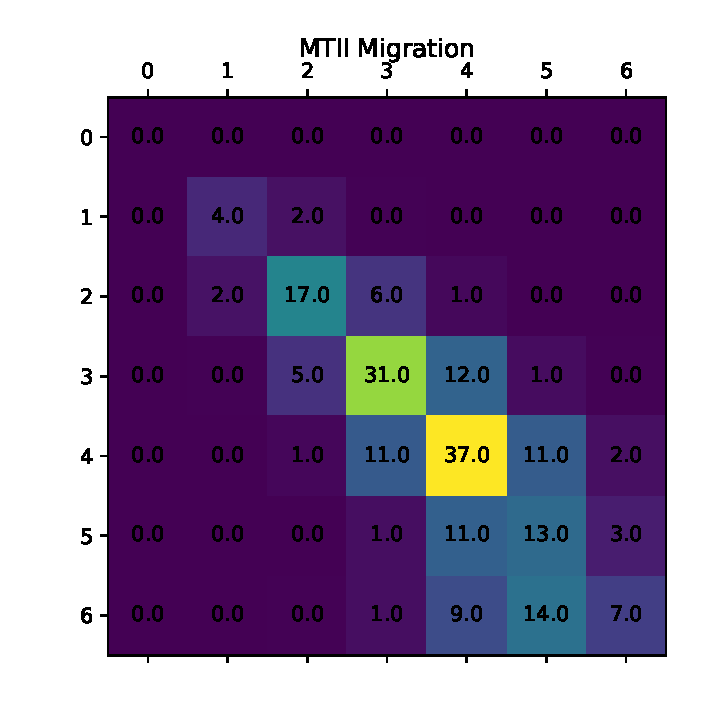
\includegraphics[width=.4\textwidth]{Pictures/unfolding/response_matrices/MTll_migrations.pdf}
  }\hfill
  \subfloat[$\Delta Y_{\ell\ell}$]{
      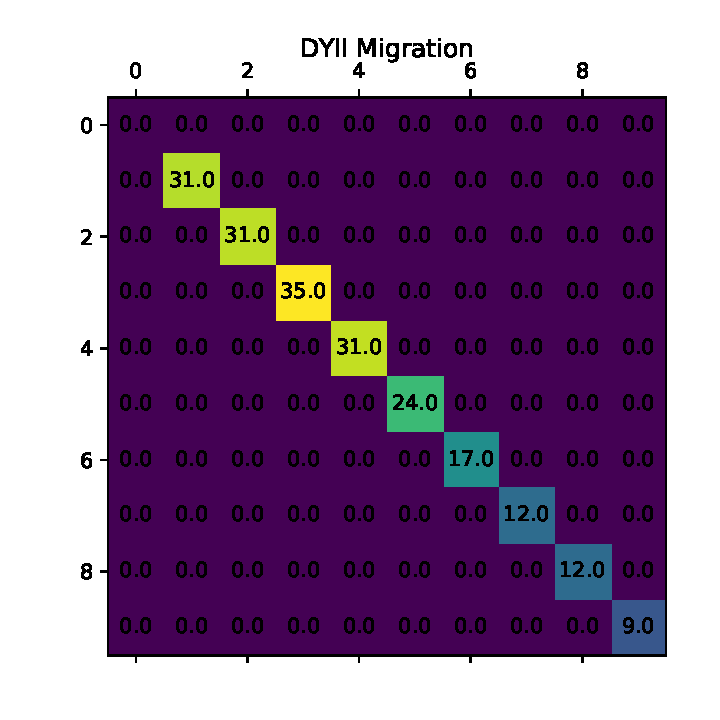
\includegraphics[width=.4\textwidth]{Pictures/unfolding/response_matrices/DYll_migrations.pdf}
  }\hfill
  \subfloat[$m_{jj}$]{
      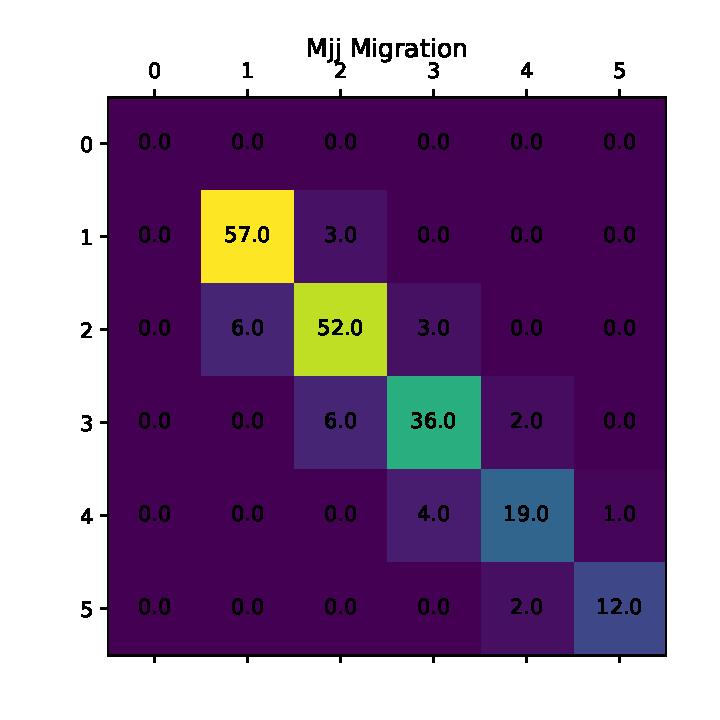
\includegraphics[width=.4\textwidth]{Pictures/unfolding/response_matrices/Mjj_migrations.pdf}
  }%hfill
\caption{\label{fig:unfoldingmatrices}Unfolding matrices shown for $p^T_H$, $m_T^{\ell\ell}$, $\Delta Y_{\ell\ell}$ and $m_{jj}$ distributions. Each bin value corresponds to normalized Bayesian probabilities and the x-axis represents reconstruction-level distributions while the y-axis shows truth distributions. **}
\end{figure}  

Further developments in unfolding are underway currently and include estimating error added by the procedure (both statistical and systematic in the case of potential mismodelling), testing for potential biases toward the truth distribution, and understanding unfolding reconstruction level uncertainties as well as nominal distributions. 

\section{Future results and measurements}

This thesis detailed the HWW VBF fiducial cross-section analysis as it currently stands, but there are further developments still underway. This analysis plans to measure differential cross-sections and the full unfolding procedure is almost complete. In addition, Chapter 5 discussed some theoretical uncertainties (VBF and ggF Higgs as well as top, WW, and $Z\rightarrow \tau\tau$) but these have not been added to the overall statistical fit. These additional uncertainties are expected to play a significant role in the overall results, particularly the large shower uncertainties. 

Signal and background yields will be used within the unfolding mechanism to extract final differential distributions. The variables used in the differential analysis will also be finalized in coming months. We aim to unfold 14 variables which are listed with their planned bin edges in \ref{tab:observablebins}. These variables probe the kinematics of the final state particles measured through this channel and add sensitivity to the total fiducial and inclusive cross-sections. The invariant mass of the two jets that accompany the $W$ bosons ($m_{jj}$) and the angular separation between them ($\Delta y_{jj}$) are particularly sensitive to the electroweak symmetry breaking mechanism. Deviations between data and theoretical predictions in the distribution of these variables may be signs of new physics that alter the HWW coupling, like new resonances at high energy scales not accessible by direct searches.                

\begin{table}[h!]
\begin{center}
\begin{tabular}{ |c||c|  }
 \hline
 Observable & Bin Edges\\
 \hline
 $MT^{l,l,MET}$ &15,40,65,80,95,110,115,120,180\\
 $Mll$&  0,20,25,30,35,40,45, 50, 60, 70,200\\
 $Mjj$ &200,450,700,950,1200,1500,2200,3000,5000\\
 $Cos(\theta^{*})$ &0,0.125,0.25,0.375,0.5,0.625,1.0\\
 $DYll$&   0,0.15,0.3,0.45,0.6,0.75,0.9,1.05,1.2,1.5,4\\
 $DYjj$& 0,2.5,3.25,3.62,4,4.35,4.75,5,5.5,6.25,7,8.5\\
 $P_{t}$ Total& 150,200,250,350,500,600,900\\
 $DPhill$& 0,0.1,0.2,0.3,0.4,0.6,0.8,1.0,1.3,1.7,2.1,2.6,3.2\\
 $P_{t} ll$&0,20,40,50,60,70,80,90,100,120,160,500\\
 Higgs $P_{t}$&0,45,80,120,160,200,260,350,1000\\
 Leading Lepton $P_{t}$&20,25,35,42,50,65,80,90,2000\\
 Subleading Lepton $P_{t}$&20,25,35,42,50,65,80,90,2000\\
 Leading Jet $P_{t}$&30,60,90,120,190,260,350,500\\
 Subleading Jet $P_{t}$& 30,60,90,120,190,260,350\\
 \hline
\end{tabular}
\end{center}
\caption{Planned observables and bin edges for differential cross-section measurements}
\label{tab:observablebins}
\end{table}

This analysis uses the full Run-2 dataset for VBF HWW cross-sections and new statistical methods. These have led to expected results which show that large increases in sensitivity with respect to the most recent Run-1 measurements. The VBF differential cross-sections measured for $H\rightarrow WW^*\ell\nu\ell\nu$ will be the first analyzed with the ATLAS experiment. 

%This analysis has an additional motivation as well. It is the first step in a larger measurement of both the VBF HWW differential cross-section and the Standard Model VBF $W+jj$ production cross-section. In the $W+$ jets production in the $\ell+$jets final state, the invariant mass of the two jets that accompany the $W$ bosons and the rapidity separation between them are particularly sensitive to the electroweak symmetry breaking mechanism just as in the VBF HWW cross-section. The final-state jets also have similar kinematics. Therefore the ratio of cross sections measurement allows for the cancellations of correlated systematic uncertainties. As both process are characterized by large ($10\%-20\%$) jet-related uncertainties, a reduction via the ratio cancellation would greatly improve the sensitivity to the VBF Higgs process and to the search for new phenomena in the context of EFT. This ratio measurement falls beyond the scope of this thesis but represents a complementary motivation to the measurements shown here. 

%In the context of vector boson scattering and with minimal assumptions on new physics, new phenomena are expected at a scale ($\Lambda$) higher than the one accessible by the experiment. These simultaneously effect $HWW$ and $WWV$ vertices. In particular, dimension-6 operators affect VBF Higgs mechanisms and VBF $W$ production, while the interplay of VBF and VBS mechanisms allows for the probe of dimension-6 and dimension-8 operators. The sensitivity to new physics is enhanced with precision-level measurements of fiducial and differential ratios of cross sections. Specifically, new phenomena that simultaneously affect both vertices are suppressed in the ratio of VBF Higgs to VBF $Wjj$ production, thus enhancing the sensitivity the phenomena affecting the $WWV$ vertex, for example. Similarly enhanced sensitivity can be achieved for anomalous quadruple-gauge couplings via the study of VBF Higgs and VBS $W$ productions. This ratio measurement between the two cross-sections is planned after publication of the VBF HWW differential cross-sections.

